\documentclass[aspectratio=169,10pt]{beamer}

\usetheme{Madrid}
\usecolortheme{default}
\setbeamertemplate{navigation symbols}{}
\setbeamertemplate{footline}[frame number]

\usepackage{amsmath,amssymb,amsthm,booktabs,mathtools}
\usepackage{stmaryrd}
\usepackage{fontspec}
\usepackage{xeCJK}
\usepackage{graphicx}
\usepackage{hyperref}
\usepackage{tikz}
\usepackage{pgfplots}
\usetikzlibrary{arrows.meta,positioning,decorations.pathreplacing,calc,fit,matrix}
\pgfplotsset{compat=1.18}

\IfFontExistsTF{Microsoft YaHei}{
  \setCJKmainfont{Microsoft YaHei}
  \setCJKsansfont{Microsoft YaHei}
}{
  \setCJKmainfont{SimSun}
  \setCJKsansfont{SimSun}
}

\definecolor{positive}{HTML}{0173B2}
\definecolor{negative}{HTML}{A65D00}
\definecolor{emphasis}{HTML}{027A5B}
\definecolor{neutral}{HTML}{666666}
\definecolor{cbPurple}{HTML}{9B5AA0}
\newcommand{\pos}[1]{\textcolor{positive}{#1}}
\newcommand{\con}[1]{\textcolor{negative}{#1}}
\newcommand{\HL}[1]{\textcolor{emphasis}{#1}}
\newcommand{\stage}[1]{\textbf{Stage~#1}}
\newcommand{\keyline}[1]{\vfill\centering\HL{\textbf{#1}}}

\setbeamercolor{structure}{fg=positive}
\setbeamercolor{alerted text}{fg=negative}
\setbeamercolor{example text}{fg=emphasis}
\setbeamerfont{frametitle}{series=\bfseries}
\setbeamerfont{block title}{series=\bfseries}

\tikzset{
  flowbox/.style={draw, rounded corners=2pt, thick, align=center,
    minimum height=0.82cm, font=\small, fill=positive!9},
  warmbox/.style={flowbox, draw=negative, fill=negative!9},
  greenbox/.style={flowbox, draw=emphasis, fill=emphasis!9},
  purplebox/.style={flowbox, draw=cbPurple, fill=cbPurple!9},
  arr/.style={-{Stealth[length=2.2mm]}, thick, draw=neutral},
  strongarr/.style={-{Stealth[length=2.4mm]}, thick, draw=positive},
  dot/.style={circle, fill=positive, inner sep=2.2pt},
  hollowdot/.style={circle, draw=negative, fill=white, thick, inner sep=2.2pt}
}

\title{参数重要性研究：后续工作流程与阶段计划}
\author{}
\institute{}
\date{2026年8月20日}

\ifdefined\SHOWPRESENTERNOTES
  \setbeameroption{show notes on second screen=right}
\else
  \setbeameroption{hide notes}
\fi

\begin{document}

% 01
\begin{frame}[plain]
  \centering
  {\LARGE\bfseries 参数重要性研究\par}
  \vspace{4pt}
  {\Large 后续工作流程与阶段计划\par}
  \vspace{12pt}
  \begin{tikzpicture}[node distance=1.25cm]
    \node[flowbox, text width=2.7cm] (estimate) {可信数值估计};
    \node[greenbox, text width=2.7cm, right=of estimate] (validate) {功能性干预};
    \node[purplebox, text width=2.7cm, right=of validate] (explain) {机制性解释};
    \draw[strongarr] (estimate) -- (validate);
    \draw[strongarr] (validate) -- (explain);
  \end{tikzpicture}
  \vfill
  {\small 2026 年 8 月 20 日}
  \note{
    本次汇报说明 Stage 1--9 的研究设计与证据依赖。全篇讨论的是后续拟开展的工作；图中的曲线、热力图和效应区间只表示计划采用的分析形式，不包含尚未获得的实验结果。\par
    本项目所说的“参数重要性”，是参数对损失变化或任务性能的可测贡献，不等同于参数绝对值、梯度幅度或某一次排序分数。研究将依次建立三类证据：估计量在统计和数值上可信；定向剪枝能够检验排序的功能后果；训练轨迹能够支持对结构形成过程的解释。\par
    汇报的核心问题是：能否构造一种可复核的参数重要性度量，并证明该度量在不同模型规模、训练路线和评价任务上具有稳定的功能含义。
  }
\end{frame}

% 02
\begin{frame}{核心研究问题｜数值排序能否代表功能重要性？}
  \begin{columns}[T]
    \column{0.47\textwidth}
      \textbf{观察到的排序}
      \begin{center}
      \begin{tikzpicture}[x=0.72cm,y=0.72cm]
        \foreach \y/\lab/\w in {3.2/$\theta_a$/5.2,2.2/$\theta_b$/3.8,1.2/$\theta_c$/2.3} {
          \node[left, font=\small] at (0,\y) {\lab};
          \draw[fill=positive!22, draw=positive, thick] (0.25,\y-0.23) rectangle (\w,\y+0.23);
        }
        \node[font=\small, text=neutral] at (3,0.35) {重要性分数（示意）};
      \end{tikzpicture}
      \end{center}
    \column{0.47\textwidth}
      \textbf{尚需补充的功能证据}
      \begin{center}
      \begin{tikzpicture}[x=0.78cm,y=0.78cm]
        \draw[-{Stealth}, thick] (0,0) -- (5.7,0) node[right, font=\small] {剪枝比例};
        \draw[-{Stealth}, thick] (0,0) -- (0,4.2) node[above, font=\small] {任务损伤};
        \draw[positive, thick] plot[smooth, domain=0:5.2] (\x,{0.13*\x*\x});
        \draw[negative, thick, dashed] plot[smooth, domain=0:5.2] (\x,{0.42*\x});
        \node[font=\small, text=positive, anchor=west] at (3.7,3.4) {高重要性};
        \node[font=\small, text=negative, anchor=west] at (3.7,1.4) {低重要性};
      \end{tikzpicture}
      \end{center}
  \end{columns}
  \begin{alertblock}{从数值排序到功能结论}
    随机梯度噪声、数值近似和训练路径均可能改变排序。只有对参数实施受控干预并测量任务损伤，才能判断排序是否反映功能差异。
  \end{alertblock}
  \note{
    左图表示估计器产生的参数排序。分数较高只说明该参数在给定定义、样本和数值近似下取得较大估计值，尚不能推出删除该参数一定造成更大性能下降。\par
    右图使用剪枝作为功能性干预。横轴“剪枝比例”是被置零或屏蔽的参数占比；纵轴“任务损伤”是剪枝模型相对未剪枝基线的性能下降，例如准确率下降或损失上升。若高重要性参数的损伤曲线稳定高于随机基线和低重要性曲线，排序才获得功能证据。\par
    随机梯度方差可能夸大分数，路径求积误差可能改变参数间次序，训练路线也可能改变重要性结构。因此，排序相关性属于描述性证据，剪枝损伤属于干预性证据，二者的结论强度不同。图中曲线仅为判读示意，不预设实验结果。
  }
\end{frame}

% 03
\begin{frame}{Stage 1--9｜从数值估计到功能证据}
  \centering
  \begin{tikzpicture}[x=1cm,y=1cm]
    \foreach \x/\n/\lab/\col in {
      0/1/实现正确/positive,
      1.55/2/估计可靠/positive,
      3.10/3/积分可靠/positive,
      4.65/4/流程验证/emphasis,
      6.20/5/规模轨迹/emphasis,
      7.75/6/范式比较/cbPurple,
      9.30/7/功能验证/cbPurple,
      10.85/8/稳健性/negative,
      12.40/9/证据整合/negative} {
      \node[draw=\col, fill=\col!9, rounded corners=2pt, thick,
        minimum width=1.28cm, minimum height=1.05cm, align=center, font=\footnotesize] (s\n) at (\x,1.6)
        {\textbf{S\n}\\\lab};
    }
    \foreach \a/\b in {1/2,2/3,3/4,4/5,5/6,6/7,7/8,8/9}
      \draw[arr] (s\a) -- (s\b);
    \draw[decorate, decoration={brace, amplitude=5pt, mirror}, thick, positive]
      (-0.65,0.85) -- (3.75,0.85) node[midway, below=8pt, font=\small] {测量可信};
    \draw[decorate, decoration={brace, amplitude=5pt, mirror}, thick, emphasis]
      (4.0,0.85) -- (6.85,0.85) node[midway, below=8pt, font=\small] {流程与规模};
    \draw[decorate, decoration={brace, amplitude=5pt, mirror}, thick, cbPurple]
      (7.1,0.85) -- (9.95,0.85) node[midway, below=8pt, font=\small] {范式与功能};
    \draw[decorate, decoration={brace, amplitude=5pt, mirror}, thick, negative]
      (10.2,0.85) -- (13.05,0.85) node[midway, below=8pt, font=\small] {稳健性与整合};
  \end{tikzpicture}
  \vspace{6pt}
  \begin{center}
  \begin{tabular}{cl}
    \toprule
    章节 & 本章要解决的问题 \\
    \midrule
    一 & 目标量、估计器与路径积分是否满足可信度要求？ \\
    二 & 完整分析流程能否扩展至更大模型与更长训练轨迹？ \\
    三 & 重要性结构能否解释训练差异并预测剪枝损伤？ \\
    四 & 主要结论是否稳健，且能够由证据逐项复核？ \\
    \bottomrule
  \end{tabular}
  \end{center}
  \note{
    九个阶段按照证据依赖组织。Stage 1 检查实现与数学定义的一致性；Stage 2 比较 raw、double sample 与 U-statistic 的统计性质；Stage 3 选择路径积分的数值求积规则。前三个阶段共同决定测量是否可信。\par
    Stage 4 在约 1.6 亿参数模型上验证训练、重要性记录、结构分析、路线比较和剪枝评价的完整流程；Stage 5 扩展至约 4.1 亿参数模型，并研究重要性随训练时间的变化。Stage 6--7 分别建立训练路线的配对比较和功能性剪枝检验，Stage 8--9 则界定稳健性范围并形成统一的结论—证据映射。\par
    阶段间的推进条件是预先规定的误差、稳定性或功能性判据。所谓 Gate，是科学决策门槛，而非行政进度节点；未满足门槛时只修正受影响环节，不将模型规模本身视为推进依据。
  }
\end{frame}

% 04
\begin{frame}{第一章｜测量可信度：实现、统计与数值核验}
  \centering
  \begin{tikzpicture}[node distance=1.55cm]
    \node[flowbox, text width=3.0cm] (s1) {\stage{1}\\实现一致性};
    \node[flowbox, text width=3.0cm, right=of s1] (s2) {\stage{2}\\统计可靠性};
    \node[flowbox, text width=3.0cm, right=of s2] (s3) {\stage{3}\\数值精度};
    \draw[strongarr] (s1) -- node[above=4pt, font=\footnotesize] {排除实现误差} (s2);
    \draw[strongarr] (s2) -- node[above=4pt, font=\footnotesize] {控制统计误差} (s3);
  \end{tikzpicture}
  \vspace{14pt}
  \begin{tikzpicture}
    \draw[thick, neutral] (0,0) -- (11.5,0);
    \foreach \x/\lab/\desc in {0/目标/定义待估量,5.75/对照/独立基准,11.5/决策/推进条件} {
      \fill[positive] (\x,0) circle (3.5pt);
      \node[above=5pt, font=\small, text=positive] at (\x,0) {\textbf{\lab}};
      \node[below=5pt, font=\small] at (\x,0) {\desc};
    }
  \end{tikzpicture}
  \keyline{分别核验实现误差、统计误差与数值误差，构成后续解释的可信度基础。}
  \note{
    第一章区分三类来源不同的误差。实现误差是代码、并行聚合或损失缩放与数学定义不一致；统计误差是有限样本造成的偏差与方差；数值误差是用有限节点近似连续路径积分所产生的截断误差和浮点误差。三类误差不能用同一项相关系数代替检验。\par
    Stage 1 固定目标量，并以独立 oracle 检查公式实现、张量运算和并行语义。Stage 2 在相同梯度预算下比较估计器的 Bias、Variance、MSE 与排序恢复能力。Stage 3 以高精度参考和完备性误差选择求积规则。\par
    这种分层核验使异常具有可定位性：解析样例失败通常指向实现；重复均值偏离参考指向统计偏差；节点增加后结果持续变化则指向求积精度不足。只有三层均满足判据，后续模型规模和功能实验才具有可解释性。
  }
\end{frame}

% 05
\begin{frame}{Stage 1｜局部梯度空间贡献的估计目标}
  \begin{columns}[T]
    \column{0.54\textwidth}
      \begin{block}{固定参数状态下的局部梯度空间贡献}
        \[
          \widehat C^{U}_{k,t}
          =\eta_{g(k),t}\,
          \frac{S_{1,k,t}^{2}-S_{2,k,t}}{M(M-1)}
        \]
      \end{block}
      \begin{itemize}
        \item $S_{1,k,t}$：$M$ 个 microbatch 梯度之和
        \item $S_{2,k,t}$：对应梯度平方和
        \item 去除对角项：目标指向总体梯度平方
      \end{itemize}
    \column{0.42\textwidth}
      \centering
      \begin{tikzpicture}[node distance=0.62cm]
        \node[flowbox, text width=3.1cm] (mb) {$M$ 个 microbatch\\梯度 $g_{1,k},\ldots,g_{M,k}$};
        \node[flowbox, text width=3.1cm, below=of mb] (ss) {充分统计量\\$S_1,\ S_2$};
        \node[greenbox, text width=3.1cm, below=of ss] (u) {去对角 U-statistic\\$\widehat C^U_{k,t}$};
        \draw[arr] (mb) -- (ss);
        \draw[strongarr] (ss) -- (u);
      \end{tikzpicture}
      \vspace{5pt}
      {\small 与参数绝对值、移动量、raw 分数并列比较}
  \end{columns}
  \keyline{本阶段验证实现与数学定义的一致性，不据此推断模型机制。}
  \note{
    本页定义固定参数状态 $\Theta_t$ 下的局部梯度空间贡献。下标 $k$ 表示参数坐标，$t$ 表示训练步；$g_{m,k,t}$ 是第 $m$ 个 microbatch 对参数 $k$ 的梯度。microbatch 是一次前向与反向传播处理的样本子集，多个 microbatch 可累积为一次 optimizer update。\par
    $M$ 是一次估计所用的 microbatch 数，$S_{1,k,t}=\sum_m g_{m,k,t}$ 为梯度和，$S_{2,k,t}=\sum_m g_{m,k,t}^2$ 为梯度平方和。恒等式 $S_1^2-S_2=\sum_{m\ne n}g_mg_n$ 删除了同一 microbatch 梯度与自身相乘的对角项，仅保留不同 microbatch 的交叉乘积。\par
    $\eta_{g(k),t}$ 是参数 $k$ 所属优化器参数组在第 $t$ 步的学习率。该系数使局部分数与优化步尺度相关，但它并不包含 AdamW 的动量、二阶矩、权重衰减和裁剪等完整效应，因此不能与 Stage 3 的实际端点路径贡献混同。\par
    单次 U-statistic 可以为负，因为有限样本中的交叉乘积可能为负；无偏性是对重复抽样期望的性质，不要求每次估计非负。若在聚合前将负值截断为零，会改变估计量的期望并引入新的正偏。
  }
\end{frame}

% 06
\begin{frame}{Stage 1｜以独立参考逐层核验实现}
  \centering
  \begin{tikzpicture}[node distance=0.78cm]
    \node[flowbox, text width=2.55cm] (a) {解析测试样例\\FP64 枚举};
    \node[flowbox, text width=2.55cm, right=of a] (b) {张量内核\\raw / double / U};
    \node[greenbox, text width=2.55cm, right=of b] (c) {Pythia-14M\\固定样本};
    \node[purplebox, text width=2.55cm, right=of c] (d) {单卡 / 多卡\\尺度一致};
    \draw[arr] (a) -- (b);
    \draw[arr] (b) -- (c);
    \draw[arr] (c) -- (d);
  \end{tikzpicture}
  \vspace{8pt}
  \begin{center}
  \begin{tabular}{lll}
    \toprule
    核验层 & 主要比较对象 & 要排除的错误 \\
    \midrule
    梯度尺度 & 完整 batch vs. microbatch & loss reduction / token 权重 \\
    估计器内核 & 显式成对式 vs. 流式式 & 对角项、分母、权重 \\
    训练接线 & 开启统计 vs. 关闭统计 & 训练轨迹被扰动 \\
    并行语义 & 相同 global batch & 聚合与累积尺度漂移 \\
    \bottomrule
  \end{tabular}
  \end{center}
  \keyline{逐张量对照独立 oracle，避免聚合结果掩盖局部实现误差。}
  \note{
    oracle 指独立于被测实现、可用于判定正确性的参考结果。独立性非常重要：若参考程序复用同一张量内核、同一分母或同一聚合逻辑，两套实现可能共享错误而仍然彼此一致。这里采用可人工核算的解析测试样例，并在 FP64 双精度浮点格式下显式枚举全部交叉乘积作为第一层 oracle；FP64 相比常见训练精度具有更小的舍入误差，适合生成数值参考。\par
    第二层检查 raw、double sample 与 U-statistic 的张量内核，重点比较逐参数结果，而非仅比较全局和。全局聚合可能因正负误差相互抵消而看似正确。第三层在 Pythia-14M 的真实参数张量上检查维度、参数组和数据类型；Pythia-14M 是约 1,400 万参数的开放语言模型，用于低成本实现验证。\par
    第四层检查训练接线和并行语义。global batch 是一次参数更新实际覆盖的全部样本，可能由多个 microbatch、多个梯度累积步和多张 GPU 共同组成。loss reduction 指损失在样本或 token 维度上采用求和还是求平均；不同 reduction 会改变梯度整体尺度。有效 token 权重用于排除 padding，并使不同长度序列按实际参与损失的 token 数聚合。相同 global batch 的单卡与分布式结果应保持同一缩放尺度。\par
    通过判据包括逐张量最大绝对误差、相对误差、归一化后误差和排序一致性。Pearson 或 Spearman 相关系数只能说明整体趋势或排序相近，不能排除统一倍数、分母错误或少量坐标的严重偏差。
  }
\end{frame}

% 06b
\begin{frame}{Stage 1｜double sample 与 U-statistic 的无偏化机制}
  \textbf{偏差来源：同一随机梯度的自乘项将抽样方差并入目标。}
  \vspace{3pt}
  \begin{columns}[T]
    \column{0.48\textwidth}
      \begin{block}{double sample｜独立样本组交叉相乘}
        \[
          \begin{aligned}
            \widehat{\mu_k^2}^{\,\mathrm{double}}
              &=\bar g_k^{(A)}\bar g_k^{(B)},\\
            \mathbb E[\widehat{\mu_k^2}^{\,\mathrm{double}}]
              &=\mu_k^2
          \end{aligned}
        \]
      \end{block}
      \begin{itemize}
        \item A、B 独立：乘积期望可分解
        \item 代价：需要两组独立梯度
      \end{itemize}
    \column{0.48\textwidth}
      \begin{block}{U-statistic｜删除同一样本的自乘项}
        \[
          \begin{aligned}
            \widehat{\mu_k^2}^{\,U}
              &=\frac{\sum_{m\ne n}g_{m,k}g_{n,k}}{M(M-1)},\\
              &=\frac{S_{1,k}^2-S_{2,k}}{M(M-1)}
          \end{aligned}
        \]
      \end{block}
      \begin{itemize}
        \item $S_1^2$ 包含全部两两乘积，$S_2$ 为自乘项之和
        \item 复用同一梯度池；单次估计可能为负
      \end{itemize}
  \end{columns}
  \vspace{3pt}
  \centering
  \begin{tikzpicture}[node distance=0.85cm]
    \node[warmbox, text width=3.2cm] (raw) {raw\\同一样本梯度自乘};
    \node[greenbox, text width=3.5cm, right=of raw] (double) {double\\两组独立梯度交叉相乘};
    \node[greenbox, text width=3.5cm, right=of double] (u) {U-statistic\\仅保留 $m\ne n$ 交叉项};
    \draw[arr] (raw) -- (double);
    \draw[arr] (double) -- (u);
  \end{tikzpicture}
  \keyline{两种估计器均以独立交叉乘积替代同一样本的随机梯度自乘。}
  \note{
    设单个梯度观测为 $g_{m,k}=\mu_k+\varepsilon_{m,k}$，其中 $\mathbb E[\varepsilon_{m,k}]=0$、$\operatorname{Var}(\varepsilon_{m,k})=\sigma_k^2$。raw estimator 对同一批平均梯度平方，展开后包含 $m=n$ 的自乘项；其期望含有 $\mathbb E[g_{m,k}^2]=\mu_k^2+\sigma_k^2$，因此抽样方差进入估计目标。\par
    double sample 将数据划分为相互独立的 A、B 两组，分别计算 $\bar g_k^{(A)}$ 与 $\bar g_k^{(B)}$。在独立性条件下，$\mathbb E[\bar g_k^{(A)}\bar g_k^{(B)}]=\mathbb E[\bar g_k^{(A)}]\mathbb E[\bar g_k^{(B)}]=\mu_k^2$。它避免了同一样本自乘，但在固定数据预算下，每组仅使用部分样本，方差和计算组织方式需要单独评估。\par
    U-statistic 在同一组 $M$ 个 microbatch 梯度中平均所有 $m\ne n$ 的有序交叉对。由于 $S_{1,k}^2$ 等于全部自乘项与交叉项之和，减去 $S_{2,k}$ 后恰好只剩交叉项；分母 $M(M-1)$ 是有序交叉对数量。该形式可用两个充分统计量流式计算，不必显式保存 $O(M^2)$ 个乘积。\par
    无偏性要求不同样本或 microbatch 在给定参数状态下独立、同分布，或至少满足使交叉协方差为零的条件。若数据存在相关性、重复样本或分布不一致，double 与 U 的期望都可能出现协方差项。两者的理论期望相同，但有限样本方差、显存占用和额外梯度成本不同，因此 Stage 2 仍需在相同预算下比较。
  }
\end{frame}

% 07
\begin{frame}{Stage 2｜raw estimator 的系统性正偏}
  \begin{columns}[T]
    \column{0.50\textwidth}
      \textbf{同一批数据同时提供两个梯度因子}
      \[
        \mathbb E[\bar g_k^2]
        =\mu_k^2+\frac{\sigma_k^2}{B}
      \]
      \begin{itemize}
        \item 目标：$\mu_k^2$
        \item 额外项：同一样本梯度的抽样方差
        \item 预测：正偏随 batch size 按 $1/B$ 衰减
      \end{itemize}
    \column{0.46\textwidth}
      \centering
      \begin{tikzpicture}[x=0.90cm,y=0.90cm]
        \draw[-{Stealth}, thick] (0,0) -- (5.7,0) node[right, font=\small] {$1/B$};
        \draw[-{Stealth}, thick] (0,0) -- (0,4.3) node[above, font=\small] {期望分数};
        \draw[neutral, thick, dashed] (0,0.9) -- (5.2,0.9);
        \draw[positive, thick] plot[domain=0:5.1] (\x,{0.9+0.50*\x});
        \foreach \x in {0.6,1.8,3.0,4.2,5.0} {
          \pgfmathsetmacro{\yraw}{0.9+0.50*\x}
          \fill[positive] (\x,\yraw) circle (2.5pt);
        }
        \node[font=\small, text=neutral, anchor=west] at (3.5,0.55) {$\mu_k^2$};
        \node[font=\small, text=positive, anchor=west] at (3.25,3.35) {raw（示意）};
      \end{tikzpicture}
      \vspace{3pt}
      {\small 图示表达预注册理论趋势，不代表已有结果。}
  \end{columns}
  \keyline{Stage 2 量化抽样方差造成的正偏，并检验其随 batch size 的衰减规律。}
  \note{
    设单样本梯度 $g_k(z)$ 的总体均值为 $\mu_k$、总体方差为 $\sigma_k^2$，一个 batch 含 $B$ 个独立同分布样本。平均梯度 $\bar g_k$ 的方差为 $\sigma_k^2/B$，由 $\mathbb E[X^2]=\operatorname{Var}(X)+\mathbb E[X]^2$ 得到 $\mathbb E[\bar g_k^2]=\mu_k^2+\sigma_k^2/B$。额外项始终非负，因此称为系统性正偏。\par
    增大 batch size 可以按 $1/B$ 速度减小正偏，但不能改变 raw estimator 在有限 $B$ 下有偏这一事实。增加独立重复次数只会更精确地估计这个有偏期望，并不会使其自动收敛到 $\mu_k^2$。\par
    预注册检验将横轴设为 $1/B$，因为理论预测偏差与其近似线性。实验需固定模型参数 $\Theta_t$、样本总体和损失定义，只改变 batch size；估计期间不执行 optimizer step，避免参数变化与抽样方差同时作用。若观察趋势显著偏离 $1/B$，需要检查样本相关性、损失归一化和梯度聚合尺度。
  }
\end{frame}

% 08
\begin{frame}{Stage 2｜等计算预算下的估计器比较}
  \vspace{4pt}
  \begin{center}
  \begin{tabular}{llll}
    \toprule
    方法 & 梯度因子来源 & 偏差预期 & 主要代价 \\
    \midrule
    raw & 同一批样本 & 正偏 & 最低 \\
    double sample & 两个独立半区 & 无偏 & 两组梯度 \\
    U-statistic & 同一梯度池去对角 & 无偏 & 维护充分统计量 \\
    \bottomrule
  \end{tabular}
  \end{center}
  \vspace{5pt}
  \centering
  \begin{tikzpicture}[node distance=0.60cm]
    \node[flowbox, text width=2.3cm] (m1) {14M\\三训练阶段};
    \node[flowbox, text width=2.3cm, right=of m1] (m2) {31M\\预注册确认};
    \node[greenbox, text width=3.7cm, right=of m2] (metrics) {Bias / Variance / MSE\\排序 / top-$k$ / 成本};
    \node[purplebox, text width=3.0cm, right=of metrics] (decision) {选择 U 或 double\\否则暂缓规模扩展};
    \draw[arr] (m1) -- (m2);
    \draw[arr] (m2) -- (metrics);
    \draw[strongarr] (metrics) -- (decision);
  \end{tikzpicture}
  \keyline{主估计器的选择同时依据统计误差、排序恢复能力与实际计算成本。}
  \note{
    三种方法使用配对样本与相同总梯度求值预算。raw 指未经偏差修正的基础估计器，它直接平方同一批平均梯度，计算最简单但存在正偏；double sample 使用两个独立样本组；U-statistic 在同一梯度池中删除对角项。比较时必须同时记录额外前向/反向次数、显存、通信量和壁钟时间。\par
    Bias 定义为重复估计的均值减去 oracle 参考值，反映系统误差；Variance 是估计量跨独立重复的波动；MSE 为均方误差，满足 $\mathrm{MSE}=\mathrm{Bias}^2+\mathrm{Variance}$。Spearman 相关系数评价完整排序的一致性，top-$k$ overlap 评价两个排序前 $k$ 个参数集合的交集比例。\par
    Pythia-14M 承担主要筛选实验，Pythia-31M 用于确认估计器选择是否能跨一个模型规模复现。14M 与 31M 分别表示约 1,400 万和 3,100 万参数，而不是训练 token 数。\par
    置信区间的统计单位应为独立重复、checkpoint 或独立模型实例。大量参数坐标共享同一训练状态和数据，不能被视为大量独立样本。Stage 2 只确定主估计器；路径积分的数值误差由 Stage 3 独立评估。
  }
\end{frame}

% 09
\begin{frame}{Stage 3｜基于实际更新端点的路径贡献}
  \begin{columns}[T]
    \column{0.53\textwidth}
      \textbf{固定更新前后端点与独立 probe 损失}
      \begin{align*}
        \Gamma_t(\alpha)&=\Theta_t+\alpha\Delta\Theta_t,\\
        C^{\mathrm{path},\mathcal P}_{k,t}
        &=-\Delta\theta_{k,t}\int_0^1
          \partial_k\mathcal L_{\mathcal P}(\Gamma_t(\alpha))\,d\alpha.
      \end{align*}
      \begin{itemize}
        \item 同一线性路径、同一确定性 probe
        \item 实际端点位移已包含优化器作用
        \item 不再额外乘学习率或裁剪因子
      \end{itemize}
    \column{0.43\textwidth}
      \centering
      \begin{tikzpicture}[x=1cm,y=1cm]
        \draw[strongarr] (0,1.4) -- (5.2,1.4);
        \fill[positive] (0.35,1.4) circle (3.5pt);
        \fill[emphasis] (4.85,1.4) circle (3.5pt);
        \node[above=6pt, font=\small] at (0.35,1.4) {$\Theta_t$};
        \node[above=6pt, font=\small] at (4.85,1.4) {$\Theta_{t+1}$};
        \foreach \x/\a in {1.25/0.2,2.60/0.5,3.95/0.8} {
          \draw[negative, thick] (\x,1.18) -- (\x,1.62);
          \node[below=5pt, font=\footnotesize, text=negative] at (\x,1.18) {$\alpha=\a$};
        }
        \draw[decorate, decoration={brace, amplitude=6pt, mirror}, thick, neutral]
          (0.35,0.45) -- (4.85,0.45) node[midway, below=9pt, font=\small] {同一条参数路径};
      \end{tikzpicture}
      \begin{exampleblock}{完备性检查}
        $\sum_k C_{k,t}=\mathcal L_{\mathcal P}(\Theta_t)-\mathcal L_{\mathcal P}(\Theta_{t+1})$
      \end{exampleblock}
  \end{columns}
  \note{
    $\Theta_t$ 与 $\Theta_{t+1}$ 分别是一次真实优化更新前后的参数，$\Delta\Theta_t=\Theta_{t+1}-\Theta_t$。线性路径 $\Gamma_t(\alpha)$ 用 $\alpha\in[0,1]$ 连接两个端点。该路径仅用于在固定端点之间评估损失梯度，不重新执行优化器。\par
    实际位移 $\Delta\Theta_t$ 已经包含学习率、动量或 Adam 一阶矩、二阶矩缩放、权重衰减以及梯度裁剪等作用。AdamW 是使用梯度一阶矩与二阶矩进行自适应缩放、并将权重衰减与梯度更新解耦的优化器。因此，路径贡献公式不能再次乘学习率或裁剪因子，否则会重复计算优化器效应。\par
    probe set 是一组固定、独立且不参与该次参数更新的评价样本。使用固定 probe 能使路径上不同 $\alpha$ 的梯度具有相同评价对象，并减少训练 batch 与评价 batch 共用造成的依赖。$\mathcal L_{\mathcal P}$ 表示 probe set 上的平均损失。\par
    完备性要求所有参数贡献之和等于两个端点的 probe loss 差。连续积分下这是由链式法则得到的恒等式；实际计算中的残差可来自有限求积节点、浮点累积误差和 probe 本身的抽样波动，三者需分别报告。
  }
\end{frame}

% 10
\begin{frame}{Stage 3｜求积精度与梯度计算成本}
  \begin{columns}[T]
    \column{0.52\textwidth}
      \textbf{同一条路径上的候选节点（示意）}
      \begin{center}
      \begin{tikzpicture}[x=5.2cm,y=1.15cm]
        \draw[-{Stealth}, thick] (0,0) -- (1.10,0) node[right, font=\small] {$\alpha$};
        \draw[-{Stealth}, thick] (0,0) -- (0,3.9) node[above, font=\small] {$\partial_k\mathcal L$};
        \draw[positive, thick] plot[smooth, domain=0:1] (\x,{1.0+1.2*\x+0.8*\x*\x});
        \foreach \x in {0,0.5,1} {
          \pgfmathsetmacro{\yq}{1.0+1.2*\x+0.8*\x*\x}
          \fill[positive] (\x,\yq) circle (2.6pt);
        }
        \node[font=\footnotesize, text=positive, anchor=west] at (0.48,3.45) {梯度曲线};
        \node[font=\footnotesize, text=neutral] at (0.12,0.55) {左端点};
        \node[font=\footnotesize, text=neutral] at (0.52,0.55) {中点};
        \node[font=\footnotesize, text=neutral] at (0.90,0.55) {右端点};
      \end{tikzpicture}
      \end{center}
    \column{0.44\textwidth}
      \begin{center}
      \begin{tabular}{lcc}
        \toprule
        规则 & 节点 & 成本 \\
        \midrule
        左端点 & 1 & 最低 \\
        梯形 & 2 & 低 \\
        Simpson & 3 & 中 \\
        复合/GL & 多节点 & 参考级 \\
        \bottomrule
      \end{tabular}
      \end{center}
      \vspace{5pt}
      \begin{tikzpicture}[node distance=0.48cm]
        \node[flowbox, text width=3.7cm] (tests) {完备性 + 向量误差\\排序 + top-$q$ + 层级稳定};
        \node[greenbox, text width=3.7cm, below=of tests] (pick) {在通过者中\\选择梯度求值最少者};
        \draw[strongarr] (tests) -- (pick);
      \end{tikzpicture}
  \end{columns}
  \keyline{在满足预注册精度标准的候选规则中，选择梯度求值次数最少者。}
  \note{
    数值求积用有限个 $\alpha$ 节点近似连续积分。左端点规则只计算 $\alpha=0$；梯形规则计算 $\alpha=0$ 与 $1$ 并取加权平均；Simpson 规则使用 $0$、$1/2$、$1$ 三个节点，对低阶多项式具有更高代数精度；Gauss--Legendre 在区间内部选择节点，复合求积则把区间划分为多个子区间。\par
    每个节点通常需要一次 probe set 的梯度求值，因此节点数近似决定额外计算量。精度比较同时检查标量完备性残差、逐参数贡献向量相对高精度参考的误差、Spearman 排序、top-$q$ 集合以及层级聚合结果。标量和相同并不能保证坐标级结果正确。\par
    高精度参考不能只使用同一种规则增加节点，因为同一方法族可能以相似方式收敛到错误实现。计划同时比较复合规则与 Gauss--Legendre，并检查节点加密后的结果是否稳定。\par
    默认规则是在所有判据均通过的候选中选择梯度求值次数最少者。若新模型、任务或路径曲率使误差超标，则按照预注册顺序增加节点，不在观察结果后临时选择最有利的规则。
  }
\end{frame}

% 11
\begin{frame}{第二章｜规模扩展与纵向轨迹分析}
  \centering
  \begin{tikzpicture}[node distance=1.7cm]
    \node[greenbox, text width=4.1cm] (s4) {\stage{4}｜160M\\端到端流程验证};
    \node[greenbox, text width=4.1cm, right=of s4] (s5) {\stage{5}｜410M\\训练期轨迹分析};
    \draw[strongarr] (s4) -- node[above=4pt, font=\footnotesize] {流程通过后扩展规模} (s5);
  \end{tikzpicture}
  \vspace{15pt}
  \begin{tikzpicture}[node distance=0.52cm]
    \node[flowbox, text width=2.3cm] (train) {训练};
    \node[flowbox, text width=2.3cm, right=of train] (importance) {重要性轨迹};
    \node[flowbox, text width=2.3cm, right=of importance] (analysis) {结构分析};
    \node[flowbox, text width=2.3cm, right=of analysis] (intervene) {功能干预};
    \node[purplebox, text width=2.3cm, right=of intervene] (compare) {路线比较};
    \draw[arr] (train) -- (importance);
    \draw[arr] (importance) -- (analysis);
    \draw[arr] (analysis) -- (intervene);
    \draw[arr] (intervene) -- (compare);
  \end{tikzpicture}
  \keyline{规模扩展用于检验同一测量与分析框架能否保持有效。}
  \note{
    160M 与 410M 分别表示模型约含 1.6 亿和 4.1 亿参数。参数规模影响训练成本、梯度统计的存储量和剪枝评价时间，因此不能直接在最大模型上同时调试所有环节。\par
    Stage 4 在 160M 模型上验证端到端研究流程，包括短程预训练、训练期重要性记录、层级与模块级聚合、训练路线比较以及临时剪枝评价。这里的目标是证明各环节之间的统计单位、参数坐标和评价口径一致，而不是从一个小规模实验推导最终规模结论。\par
    Stage 5 扩展至 410M 模型，并增加纵向 checkpoint，以分析重要性结构在训练早期形成、在中期分化以及在后期稳定的时间尺度。若 160M 阶段出现统计漂移、参数索引不一致或剪枝评价不可复现，问题应在 Stage 4 内解决，不直接扩大到 410M。
  }
\end{frame}

% 12
\begin{frame}{Stage 4｜160M 模型的端到端流程验证}
  \centering
  \begin{tikzpicture}[node distance=0.42cm]
    \node[flowbox, text width=2.15cm] (train) {短程预训练};
    \node[flowbox, text width=2.15cm, right=of train] (imp) {在线重要性};
    \node[flowbox, text width=2.15cm, right=of imp] (stats) {层/模块分析};
    \node[warmbox, text width=2.15cm, right=of stats] (prune) {剪枝评价};
    \node[purplebox, text width=2.15cm, right=of prune] (routes) {训练路线比较};
    \draw[arr] (train) -- (imp);
    \draw[arr] (imp) -- (stats);
    \draw[arr] (stats) -- (prune);
    \draw[arr] (prune) -- (routes);
    \draw[strongarr, rounded corners=6pt] (routes.south) -- ++(0,-0.55) -| (train.south);
    \node[font=\footnotesize, text=emphasis] at (6.25,-1.18) {异常定位 · 方法修正 · 针对性复验};
  \end{tikzpicture}
  \vspace{9pt}
  \begin{columns}[T]
    \column{0.48\textwidth}
      \begin{block}{流程验证内容}
        \begin{itemize}
          \item 训练期间能否稳定记录重要性
          \item 统计量能否支持结构分析与剪枝
          \item 训练路线是否满足受控配对条件
        \end{itemize}
      \end{block}
    \column{0.48\textwidth}
      \begin{alertblock}{本阶段的结论边界}
        \begin{itemize}
          \item 不据此形成最终规模结论
          \item 单次剪枝曲线仅用于流程校验
          \item 估计器和求积沿用前章选择
        \end{itemize}
      \end{alertblock}
  \end{columns}
  \keyline{160M 阶段用于验证流程完整性，并识别规模扩展前的系统性问题。}
  \note{
    “端到端流程”指同一模型从训练开始，依次产生 checkpoint、重要性统计、结构分析、剪枝 mask 和任务评价，并保证每一步都能追溯到相同的参数坐标与训练状态。流程验证关注接口和科学口径的一致性，不涉及服务器调度或运行合同。\par
    “在线重要性”表示在训练过程中按照预定 checkpoint 计算统计量。checkpoint 是特定训练步保存的模型状态及其关联指标；记录多个 checkpoint 可以研究时间变化，而只分析终点模型只能得到静态截面。在线计算还需验证其不会改变随机数状态、梯度累积或优化轨迹。\par
    路线比较要求共享模型架构、基础初始化、下游任务和评价流程，并明确训练预算的对齐方式。剪枝使用临时 mask，即评价时将指定参数置零或屏蔽，测量结束后恢复原权重；这样得到的是局部功能损伤，不把恢复训练或永久稀疏化的适应效应混入结果。\par
    Stage 4 的通过条件包括：重要性记录无缺失且尺度稳定；层级聚合能回溯到参数坐标；配对路线满足预定对照条件；相同 mask 的评价可复现。单一 seed 或单条曲线只验证流程，不支持普遍性结论。
  }
\end{frame}

% 13
\begin{frame}{Stage 4｜受控训练路线的初步对照}
  \centering
  \begin{tikzpicture}[node distance=0.75cm]
    \node[flowbox, text width=3.0cm] (base) {统一基础初始化};
    \node[purplebox, text width=3.1cm, below left=1.05cm and 1.1cm of base] (direct) {直接监督训练\\SST-2};
    \node[greenbox, text width=3.1cm, below right=1.05cm and 1.1cm of base] (pre) {语言模型预训练};
    \node[greenbox, text width=3.1cm, below=0.62cm of pre] (ft) {监督微调\\SST-2};
    \node[warmbox, text width=4.0cm, below=1.05cm of $(direct)!0.5!(ft)$] (compare) {配对比较\\性能 · 轨迹 · 重要性 · 剪枝损伤};
    \draw[strongarr] (base) -- (direct);
    \draw[strongarr] (base) -- (pre);
    \draw[arr] (pre) -- (ft);
    \draw[arr] (direct) -- (compare);
    \draw[arr] (ft) -- (compare);
  \end{tikzpicture}
  \vspace{3pt}
  \begin{center}
  \begin{tabular}{lll}
    \toprule
    固定条件 & 唯一核心差异 & 第一轮输出 \\
    \midrule
    架构、初始化、评价任务 & 是否经历语言模型预训练 & 可比较的流程证据 \\
    \bottomrule
  \end{tabular}
  \end{center}
  \keyline{本阶段核验配对设计，路线差异的稳定性由后续多任务实验检验。}
  \note{
    两条路线共享模型架构、基础初始化和下游评价任务。路线 A 从基础初始化直接在 SST-2 上进行监督训练；路线 B 先进行语言模型预训练，再在同一 SST-2 任务上微调。SST-2 是二分类情感分析任务，详细定义在 Stage 6 说明。\par
    核心处理变量是“是否经历语言模型预训练”。除该变量外，还需记录并尽可能控制优化器、下游数据划分、评价频率和随机 seed。若总训练计算量无法严格相等，应同时报告“相同下游预算”和“相同总计算预算”两种解释口径，避免把额外预训练计算误写成纯方法优势。\par
    配对比较指同一初始化与 seed 下的两条路线构成一对，先计算对内差值，再跨独立配对汇总。这样可以消除部分初始化难度和数据顺序差异。Stage 4 只检验配对流程、参数坐标和评价接口；正式的多任务、多 seed 统计推断在 Stage 6 完成。
  }
\end{frame}

% 14
\begin{frame}{Stage 5｜410M 模型的训练期重要性轨迹}
  \textbf{训练早期采用密集测量，随后增加相邻 checkpoint 的间隔}
  \begin{center}
  \begin{tikzpicture}[x=1cm,y=1cm]
    \draw[-{Stealth}, thick] (0,1.2) -- (13.2,1.2) node[right, font=\small] {训练进程};
    \foreach \x in {0.6,1.25,1.9,2.55,3.2,4.2,5.35,6.7,8.4,10.4,12.4} {
      \draw[positive, thick] (\x,0.95) -- (\x,1.45);
      \fill[positive] (\x,1.2) circle (2.6pt);
    }
    \draw[decorate, decoration={brace, amplitude=5pt, mirror}, thick, positive]
      (0.45,0.55) -- (3.35,0.55) node[midway, below=8pt, font=\small] {早期：密集 checkpoint};
    \draw[decorate, decoration={brace, amplitude=5pt, mirror}, thick, emphasis]
      (3.8,0.55) -- (12.65,0.55) node[midway, below=8pt, font=\small] {中后期：观察稳定与分化};
  \end{tikzpicture}
  \end{center}
  \vspace{6pt}
  \begin{center}
  \begin{tabular}{lll}
    \toprule
    每个测量点 & 时间序列聚合 & 研究问题 \\
    \midrule
    loss、梯度范数、更新范数 & 层/模块重要性 & 哪些结构先分化？ \\
    raw、U、signed/positive/negative & 集中度与有效参数数 & 重要性是否越来越集中？ \\
    参数移动量与 top-$k$ & 集合稳定性 & 关键参数何时稳定？ \\
    \bottomrule
  \end{tabular}
  \end{center}
  \note{
    checkpoint 是训练过程中某一确定步数对应的模型参数状态及关联统计。Stage 5 在多个 checkpoint 记录训练 loss、梯度范数、参数更新范数和重要性，而非只读取最终模型。纵向数据能够区分“早期出现并持续稳定”“中期形成”与“终点偶然出现”三种不同模式。\par
    训练早期的梯度和参数更新通常变化更快，因此采用更密集的测量点；中后期增加间隔以控制梯度统计成本。测量频率本身可能影响对稳定时间的判断，所以 Stage 8 将 checkpoint 频率纳入敏感性分析。\par
    loss 是模型在指定数据上的目标函数值；梯度范数衡量当前损失对参数的局部敏感度；更新范数衡量优化器实际造成的参数位移。三者与重要性同时记录，可判断重要性集中是否只是整体梯度尺度变化的结果。\par
    signed contribution 保留贡献的正负号；positive 与 negative 分别聚合正贡献和负贡献。符号对应参数位移对 probe loss 的下降或上升方向，具体解释取决于公式中的负号约定。分开报告可避免绝对值把相反作用合并为同一种“高重要性”。
  }
\end{frame}

% 15
\begin{frame}{Stage 5｜训练轨迹的三类动态结构表征}
  \begin{columns}[T]
    \column{0.31\textwidth}
      \centering
      \textbf{层 × checkpoint}
      \begin{tikzpicture}[x=0.42cm,y=0.38cm]
        \foreach \r in {0,...,5} {
          \foreach \c in {0,...,6} {
            \pgfmathtruncatemacro{\shade}{8+5*\r+4*\c}
            \fill[positive!\shade] (\c,\r) rectangle ++(0.86,0.86);
          }
        }
        \draw[thick] (0,0) rectangle (6.86,5.86);
        \node[font=\footnotesize] at (3.4,-0.7) {训练进程};
        \node[font=\footnotesize, rotate=90] at (-0.7,2.9) {深度};
      \end{tikzpicture}
      {\small 分化顺序与深度结构}
    \column{0.31\textwidth}
      \centering
      \textbf{集中度轨迹}
      \begin{tikzpicture}[x=0.52cm,y=0.52cm]
        \draw[-{Stealth}, thick] (0,0) -- (5.4,0);
        \draw[-{Stealth}, thick] (0,0) -- (0,4.2);
        \draw[emphasis, thick] plot[smooth, domain=0:5] (\x,{0.65+2.6*(1-exp(-0.55*\x))});
        \node[font=\footnotesize, text=emphasis] at (3.5,3.55) {Gini / HHI};
        \node[font=\footnotesize] at (2.6,-0.55) {训练进程};
      \end{tikzpicture}
      {\small 重要性是否聚集}
    \column{0.31\textwidth}
      \centering
      \textbf{top-$k$ 稳定性}
      \begin{tikzpicture}[x=0.52cm,y=0.52cm]
        \draw[-{Stealth}, thick] (0,0) -- (5.4,0);
        \draw[-{Stealth}, thick] (0,0) -- (0,4.2);
        \draw[cbPurple, thick] plot[smooth, domain=0:5] (\x,{0.45+3.1*(1-exp(-0.65*\x))});
        \draw[neutral, dashed, thick] (0,3.45) -- (5.0,3.45);
        \node[font=\footnotesize, text=cbPurple] at (3.4,3.0) {overlap};
        \node[font=\footnotesize] at (2.6,-0.55) {训练进程};
      \end{tikzpicture}
      {\small 关键集合何时稳定}
  \end{columns}
  \vspace{8pt}
  \centering{\small 所有图均为计划输出结构示意；正式数值由 Stage 5 实验产生。}
  \keyline{将逐参数时间序列转化为层级结构、集中度与集合稳定性表征。}
  \note{
    左侧热力图以层或模块为纵轴、checkpoint 为横轴，颜色表示该层聚合后的重要性。它用于识别不同深度、注意力模块与前馈模块的分化顺序。聚合前需明确使用总和、均值还是参数数量归一化，否则大模块可能仅因参数更多而取得更大数值。\par
    中间的 Gini coefficient 衡量归一化重要性分布的不均衡程度。对非负份额而言，Gini 为 0 表示所有参数份额完全相等，数值接近 1 表示重要性集中在极少数参数上。它对分布整体形状敏感，但不能直接指出由哪些参数承担。\par
    HHI 是 Herfindahl--Hirschman Index。令非负归一化份额为 $p_k$ 且 $\sum_k p_k=1$，则 $\mathrm{HHI}=\sum_k p_k^2$。HHI 越大，重要性越集中；有效参数数定义为 $N_{\mathrm{eff}}=1/\mathrm{HHI}$，可解释为产生同等集中度的等权参数数量。entropy 为 $-\sum_k p_k\log p_k$，数值越大表示分布越分散，其方向与 HHI 相反。\par
    top-$k$ overlap 比较两个 checkpoint 前 $k$ 个参数集合的交集比例；若需校正随机重合，还应同时给出随机基线或 Jaccard index。完整排序则使用 Spearman 相关系数。Gini、HHI、entropy 和 top-$k$ 回答不同问题，不能互相替代。
  }
\end{frame}

% 16
\begin{frame}{第三章｜训练路线差异与功能性验证}
  \centering
  \begin{tikzpicture}[node distance=1.6cm]
    \node[purplebox, text width=4.0cm] (s6) {\stage{6}｜路线比较\\训练路线留下了什么差异？};
    \node[purplebox, text width=4.0cm, right=of s6] (s7) {\stage{7}｜功能干预\\排序能否预测功能损伤？};
    \draw[strongarr] (s6) -- node[above=4pt, font=\footnotesize] {结构差异接受剪枝检验} (s7);
  \end{tikzpicture}
  \vspace{16pt}
  \begin{tikzpicture}[node distance=0.58cm]
    \node[flowbox, text width=3.0cm] (observe) {观察\\分布与轨迹};
    \node[greenbox, text width=3.0cm, right=of observe] (hypothesis) {提出解释\\参数复用 / 分工};
    \node[warmbox, text width=3.0cm, right=of hypothesis] (intervention) {施加干预\\定向剪枝};
    \node[purplebox, text width=3.0cm, right=of intervention] (judge) {功能判别\\任务损伤};
    \draw[arr] (observe) -- (hypothesis);
    \draw[arr] (hypothesis) -- (intervention);
    \draw[strongarr] (intervention) -- (judge);
  \end{tikzpicture}
  \keyline{训练路线比较提出结构假设，定向剪枝检验其功能后果。}
  \note{
    Stage 6 的训练路线比较属于受控观察：在尽量一致的初始化、任务和预算下，比较直接监督与预训练后微调的性能和重要性结构。它可以识别稳定关联，但仅凭结构差异仍不能证明某组参数对任务功能具有因果作用。\par
    Stage 7 采用定向剪枝实施干预。若删除高重要性参数造成的性能损伤系统性大于随机剪枝，并且删除低重要性参数的损伤更小，则排序获得功能性支持。这里的“功能性”是相对于指定任务、模型状态和剪枝操作定义的，不等于一般意义上的唯一因果解释。\par
    seed 是随机数生成器的初始编号，控制参数初始化、数据打乱、dropout 和随机 mask 等过程。不同 seed 形成独立重复，用于估计结果对随机性的敏感程度。单个 seed 的终点差异可能来自偶然训练波动，因此还需比较收敛速度、参数结构和跨 seed 的置信区间。
  }
\end{frame}

% 17
\begin{frame}{Stage 6｜训练路线的受控配对设计}
  \centering
  \begin{tikzpicture}[node distance=0.65cm]
    \node[flowbox, text width=2.9cm] (base) {同一架构与初始化};
    \node[purplebox, text width=3.5cm, below left=0.85cm and 1.1cm of base] (direct) {路线 A｜直接监督\\SST-2 / MNLI / RTE};
    \node[greenbox, text width=3.5cm, below right=0.85cm and 1.1cm of base] (pre) {路线 B｜预训练 → 微调\\SST-2 / MNLI / RTE};
    \node[warmbox, text width=5.0cm, below=0.75cm of $(direct)!0.5!(pre)$] (paired) {按任务、seed 与训练预算配对比较};
    \draw[strongarr] (base) -- (direct);
    \draw[strongarr] (base) -- (pre);
    \draw[arr] (direct) -- (paired);
    \draw[arr] (pre) -- (paired);
  \end{tikzpicture}
  \vspace{5pt}
  \begin{center}
  \begin{tabular}{lll}
    \toprule
    任务角色 & 主要用途 & 压力维度 \\
    \midrule
    SST-2 & 稳定二分类对照 & 清晰、低噪声 \\
    MNLI & 主要自然语言推理 & 规模与泛化 \\
    RTE & 低资源压力测试 & 样本效率 \\
    \bottomrule
  \end{tabular}
  \end{center}
  \note{
    SST-2、MNLI 与 RTE 都属于 GLUE 语言理解基准，但任务结构和数据规模不同。SST-2 全称 Stanford Sentiment Treebank 2，是单句二分类情感任务，标签为 positive 与 negative；文本主要来自电影评论，类别定义直接，适合作为稳定的基础对照。\par
    MNLI 全称 Multi-Genre Natural Language Inference。输入是一对句子：premise（前提）与 hypothesis（假设），模型判断二者关系为 entailment（前提蕴含假设）、neutral（信息不足以判断）或 contradiction（相互矛盾）。数据覆盖多种文本体裁，可检验跨领域泛化和较复杂的句间推理。\par
    RTE 全称 Recognizing Textual Entailment，同样输入前提与假设，但通常作为二分类任务，判断是否存在蕴含关系。其训练数据明显少于 MNLI，因此更容易受到 seed 和初始化影响，适合检验预训练表示在低资源条件下的样本效率。\par
    每个任务内，两条路线按初始化、seed、数据划分、下游训练步数和评价时间点配对。最终报告既给出任务性能，也比较重要性分布、层级结构，以及预训练阶段 top-$k$ 参数在微调阶段的保留或替换程度。
  }
\end{frame}

% 18
\begin{frame}{Stage 6｜任务性能与参数结构的联合比较}
  \begin{columns}[T]
    \column{0.48\textwidth}
      \begin{block}{任务表现}
        \begin{itemize}
          \item 最终任务性能与置信区间
          \item 收敛速度与样本效率
          \item 多 seed 稳定性与泛化差异
        \end{itemize}
      \end{block}
      \centering
      \begin{tikzpicture}[x=0.60cm,y=0.52cm]
        \draw[-{Stealth}, thick] (0,0) -- (5.5,0) node[right, font=\footnotesize] {训练};
        \draw[-{Stealth}, thick] (0,0) -- (0,3.5) node[above, font=\footnotesize] {性能};
        \draw[positive, thick] plot[smooth, domain=0:5] (\x,{0.35+2.75*(1-exp(-0.72*\x))});
        \draw[negative, thick] plot[smooth, domain=0:5] (\x,{0.25+2.35*(1-exp(-0.42*\x))});
        \node[font=\footnotesize, text=positive] at (3.8,3.05) {预训练后微调};
        \node[font=\footnotesize, text=negative] at (3.9,2.1) {直接监督};
      \end{tikzpicture}
    \column{0.48\textwidth}
      \begin{block}{参数结构}
        \begin{itemize}
          \item 重要性分布与层/模块分工
          \item 集中度与有效参数数量
          \item 预训练 top-$k$ 在微调中的复用
        \end{itemize}
      \end{block}
      \centering
      \begin{tikzpicture}[node distance=0.52cm]
        \node[flowbox, text width=3.8cm] (pre) {预训练重要参数集合\\$\mathcal T_{\mathrm{pre}}$};
        \node[purplebox, text width=3.8cm, below=of pre] (ft) {微调重要参数集合\\$\mathcal T_{\mathrm{ft}}$};
        \node[greenbox, text width=3.8cm, below=of ft] (overlap) {overlap + rank correlation\\层/模块复用};
        \draw[arr] (pre) -- (ft);
        \draw[strongarr] (ft) -- (overlap);
      \end{tikzpicture}
  \end{columns}
  \centering{\small 曲线仅说明计划比较的形态，不预设哪条路线更优。}
  \note{
    任务性能根据数据集采用相应指标，例如分类准确率或验证损失。最终性能描述训练终点；收敛速度可用达到预定性能阈值所需的优化步数或样本数衡量；样本效率比较在相同标注数据量下的性能。多 seed 置信区间反映训练随机性，而不是单次运行中的 minibatch 波动。\par
    参数结构比较包括层与模块的重要性份额、Gini/HHI 等集中度指标、有效参数数，以及预训练和微调阶段前 $k$ 个参数集合的重合。Spearman rank correlation 使用秩而非原始数值，衡量完整排序的单调一致性；Pearson correlation 则衡量原始数值的线性关系。\par
    “重要性复用”是指预训练阶段获得较高重要性的同一参数坐标，在微调中仍保持较高排序或较大份额。该概念要求两阶段模型具有一一对应的参数坐标；若结构、参数命名或张量形状改变，应改用层级或模块级映射，不能直接计算逐参数 overlap。\par
    任务表现和参数结构若同时、稳定地随训练路线变化，可以支持后续机制假设；若只有性能差异而结构不变，或只有结构差异而性能不变，则需分别解释，不能合并为同一结论。
  }
\end{frame}

% 19
\begin{frame}{Stage 7｜等预算的定向剪枝对照设计}
  \begin{columns}[T]
    \column{0.62\textwidth}
      \textbf{重要性来源 × 剪除方向}
      \vspace{4pt}
      \centering
      \begin{tikzpicture}[x=1.22cm,y=0.58cm]
        \foreach \c/\lab in {0/高重要性,1/低重要性,2/随机} {
          \node[font=\footnotesize, align=center] at (3.45+\c,6.6) {\lab};
        }
        \foreach \r/\lab in {0/magnitude,1/movement,2/raw,3/U or double,4/Fisher,5/SI} {
          \node[font=\footnotesize, anchor=east] at (2.85,5.8-\r) {\lab};
          \foreach \c in {0,1,2} {
            \pgfmathtruncatemacro{\tone}{14+7*mod(\r+\c,3)}
            \draw[thick, positive!70] (3.05+\c,5.45-\r) rectangle ++(0.78,0.68);
            \fill[positive!\tone] (3.05+\c,5.45-\r) rectangle ++(0.78,0.68);
          }
        }
        \draw[thick] (3.05,-0.55) rectangle (5.83,6.13);
      \end{tikzpicture}
    \column{0.34\textwidth}
      \begin{block}{每个组合都要覆盖}
        \begin{itemize}
          \item 多个剪枝比例
          \item 全局与层内平衡
          \item 多随机 mask
          \item 语言模型与下游任务
        \end{itemize}
      \end{block}
      \begin{tikzpicture}[node distance=0.48cm]
        \node[flowbox, text width=3.5cm] (rank) {冻结排序};
        \node[warmbox, text width=3.5cm, below=of rank] (mask) {临时应用 mask};
        \node[greenbox, text width=3.5cm, below=of mask] (eval) {评价任务损伤};
        \draw[arr] (rank) -- (mask);
        \draw[strongarr] (mask) -- (eval);
      \end{tikzpicture}
  \end{columns}
  \keyline{固定评价预算、任务与剪枝比例，仅改变参数排序及剪除方向。}
  \note{
    对每一种排序方法，都分别删除高重要性参数、低重要性参数和随机参数，并在多个剪枝比例上评价。高分剪枝检验分数是否识别关键参数；低分剪枝检验分数是否识别冗余参数；随机剪枝提供不利用排序信息时的基线分布。随机 mask 需要多次独立抽样，以形成均值和置信区间。\par
    global pruning 在全模型范围内统一排序并选择参数，能够反映不同层之间的竞争；layer-balanced pruning 在每层删除相同比例，控制层大小和尺度差异。两种设置回答的问题不同，应并列报告。mask 在评价期间固定，避免每个 batch 使用不同随机结构。\par
    magnitude baseline 按权重绝对值 $|\theta_k|$ 排序；movement baseline 按训练期间的参数位移 $|\theta_{k,t}-\theta_{k,0}|$ 或其累计形式排序；Fisher baseline 使用梯度平方或 Fisher information 的对角近似衡量局部损失敏感度；SI 全称 Synaptic Intelligence，通过训练轨迹累计参数更新与损失下降的关联来估计重要性。\par
    raw、U-statistic、double sample 与传统基线必须共享模型 checkpoint、评价任务、剪枝比例和 mask 数量。若某方法需要额外梯度计算，应单独报告估计成本，使功能效果与计算代价可以同时比较。
  }
\end{frame}

% 20
\begin{frame}{Stage 7｜剪枝曲线的功能性判定标准}
  \begin{columns}[T,onlytextwidth]
    \column{0.59\textwidth}
      \centering
      \begin{tikzpicture}[x=0.88cm,y=0.78cm]
        \draw[-{Stealth}, thick] (0,0) -- (6.8,0) node[right, font=\small] {剪枝比例};
        \draw[-{Stealth}, thick] (0,0) -- (0,5.1) node[above, font=\small] {任务损伤};
        \draw[positive, thick] plot[smooth, domain=0:6.2] (\x,{0.10*\x*\x+0.12*\x});
        \draw[neutral, thick] plot[smooth, domain=0:6.2] (\x,{0.42*\x});
        \draw[negative, thick] plot[smooth, domain=0:6.2] (\x,{0.22*\x});
        \node[font=\small, text=positive, anchor=west] at (4.35,4.05) {先剪高重要性};
        \node[font=\small, text=neutral, anchor=west] at (4.35,2.35) {随机};
        \node[font=\small, text=negative, anchor=west] at (4.35,1.05) {先剪低重要性};
        \draw[decorate, decoration={brace, amplitude=5pt}, thick, cbPurple]
          (2.0,1.05) -- (2.0,0.45) node[midway, left=7pt, font=\footnotesize] {损伤差距};
      \end{tikzpicture}
      {\small 预期判别形态（示意），正式结论由重复实验给出。}
    \column{0.35\textwidth}
      \begin{block}{预注册通过条件}
        \begin{itemize}
          \item 高重要性曲线显著更陡
          \item 低重要性优于随机基线
          \item 多比例下顺序稳定
          \item AUC 差异带置信区间
        \end{itemize}
      \end{block}
      \vspace{6pt}
      \begin{alertblock}{解释边界}
        曲线不分离：仅保留描述性用途；不宣称功能有效。
      \end{alertblock}
  \end{columns}
  \note{
    若排序具有功能含义，高重要性剪枝应在相同剪枝比例下造成更大任务损伤，低重要性剪枝应小于随机基线，并且该顺序应在预先指定的一段比例范围内保持。只在单个比例出现差异，可能来自评价噪声或曲线局部波动，证据强度有限。\par
    任务损伤需要统一方向。例如以准确率为指标时，可定义为未剪枝准确率减去剪枝后准确率；以 loss 为指标时，可定义为剪枝后 loss 减去未剪枝 loss。这样数值越大始终代表功能损伤越严重。\par
    Damage AUC 是损伤函数 $D(r)$ 关于剪枝比例 $r$ 的曲线下面积，实际用预定比例节点上的梯形求积计算。AUC 将多个比例的结果汇总为一个整体指标，但仍需展示原始曲线，因为相同 AUC 可能对应不同的局部形状。\par
    高、低和随机曲线之间的 AUC 差异使用配对 seed 与随机 mask 计算置信区间。参数坐标共享模型和训练历史，不能作为独立重复。若曲线不稳定分离，结论应限定为“描述性排序”，不宣称其能够预测功能损伤。
  }
\end{frame}

% 21
\begin{frame}{第四章｜稳健性分析与证据整合}
  \centering
  \begin{tikzpicture}[node distance=1.6cm]
    \node[warmbox, text width=4.0cm] (s8) {\stage{8}｜消融与稳健性\\结论依赖什么？};
    \node[warmbox, text width=4.0cm, right=of s8] (s9) {\stage{9}｜统一分析\\怎样得到可复核的结论？};
    \draw[strongarr] (s8) -- node[above=4pt, font=\footnotesize] {界定适用范围} (s9);
  \end{tikzpicture}
  \vspace{16pt}
  \begin{tikzpicture}[node distance=0.55cm]
    \node[flowbox, text width=2.8cm] (claim) {待检验结论};
    \node[warmbox, text width=2.8cm, right=of claim] (stress) {逐项改变条件};
    \node[greenbox, text width=2.8cm, right=of stress] (boundary) {结论适用边界};
    \node[purplebox, text width=2.8cm, right=of boundary] (evidence) {结论与证据对照};
    \draw[arr] (claim) -- (stress);
    \draw[arr] (stress) -- (boundary);
    \draw[strongarr] (boundary) -- (evidence);
  \end{tikzpicture}
  \keyline{仅将跨关键因素保持稳定的结果纳入主要结论。}
  \note{
    Stage 8 通过单因素消融检验结论对实验条件的敏感性。每个子实验相对基准只改变一个预注册因素，使观察到的效应尽可能归因于该因素。分析结果分为三类：跨设置稳定、仅在特定条件下成立，以及在关键条件下发生方向反转。\par
    稳健性要求结论方向、效应量级和不确定性在合理条件变化下保持可解释，并不要求所有数值完全相同。若效应随模型规模或归一化方式显著变化，应明确报告交互关系与适用范围，避免用平均结果掩盖异质性。\par
    Stage 9 建立 claim--evidence mapping，即“结论—证据映射”。论文中的每项结论都对应具体表格、图、统计定义、实验阶段与不确定性说明。该映射用于区分直接证据、支持性证据和未覆盖范围，使另一位研究者能够沿统一口径复核结论。
  }
\end{frame}

% 22
\begin{frame}{Stage 8｜单因素消融设计}
  \begin{columns}[T,onlytextwidth]
    \column{0.63\textwidth}
      \centering
      \begin{tikzpicture}[x=1cm,y=1cm]
        \node[greenbox, text width=2.3cm] (base) at (0,0) {基准条件};
        \node[flowbox, text width=2.15cm] (batch) at (-3.4,2.1) {batch size};
        \node[flowbox, text width=2.15cm] (micro) at (0,2.1) {microbatch 数};
        \node[flowbox, text width=2.15cm] (nodes) at (3.4,2.1) {积分节点};
        \node[flowbox, text width=2.15cm] (sign) at (-3.4,0) {正/负贡献};
        \node[flowbox, text width=2.15cm] (norm) at (3.4,0) {归一化方式};
        \node[flowbox, text width=2.15cm] (scale) at (-3.4,-2.1) {模型规模};
        \node[flowbox, text width=2.15cm] (seed) at (0,-2.1) {随机 seed};
        \node[flowbox, text width=2.15cm] (data) at (3.4,-2.1) {数据规模};
        \foreach \n in {batch,micro,nodes,sign,norm,scale,seed,data}
          \draw[arr] (base) -- (\n);
      \end{tikzpicture}
    \column{0.33\textwidth}
      \begin{block}{单因素设计的作用}
        \begin{itemize}
          \item 父子实验共享其余条件
          \item 效应可归因于注册因素
          \item 避免组合变化掩盖根因
        \end{itemize}
      \end{block}
      \vspace{8pt}
      \begin{alertblock}{矩阵先定，结果后看}
        所有组合按同一规则汇总；没有运行过的组合不作外推。
      \end{alertblock}
  \end{columns}
  \keyline{消融分析用于识别结论成立的必要条件，而非单纯增加实验数量。}
  \note{
    基准条件是一组固定的默认配置，每个消融子实验只改变一个因素。batch size 是一次统计估计或优化更新覆盖的样本总量，决定平均梯度的抽样方差；microbatch size 是一次前向/反向传播处理的子批量大小，microbatch 数则决定 U-statistic 可用的交叉对数量。二者可能具有相同 global batch，却产生不同的估计结构。\par
    积分节点数量与位置控制 Stage 3 的求积截断误差。正贡献、负贡献和带符号贡献决定如何处理方向信息；归一化方式决定比较的是总质量、每参数平均值、每层份额还是相对基线变化。改变归一化可能影响跨层和跨规模结论，因此必须单独检验。\par
    模型规模检验规律能否从 160M 扩展到 410M；seed 检验随机初始化、数据顺序和 dropout 的影响；数据规模检验估计稳定性与样本效率。checkpoint 频率虽未画入矩阵，也需作为时间离散化因素评估。\par
    单因素结果应报告效应量与置信区间，而不只列显著或不显著。若两个因素可能发生交互，例如 batch size 与 microbatch 数共同影响方差，应在单因素筛选后增加有针对性的二维验证，并明确其不属于原始单因素结论。
  }
\end{frame}

% 23
\begin{frame}{Stage 8｜敏感性分析与结论适用范围}
  \begin{columns}[T,onlytextwidth]
    \column{0.57\textwidth}
      \textbf{相对基准的效应与不确定性（判读示意）}
      \begin{center}
      \begin{tikzpicture}[x=0.60cm,y=0.58cm]
        \draw[-{Stealth}, thick] (-4.2,0) -- (4.6,0);
        \draw[neutral, dashed, thick] (0,-0.45) -- (0,7.2);
        \foreach \y/\lab/\x/\lo/\hi in {
          6.5/batch/0.4/-0.4/1.2,
          5.5/microbatch/1.1/0.3/1.9,
          4.5/积分节点/-0.3/-1.1/0.5,
          3.5/归一化/2.0/1.1/2.9,
          2.5/模型规模/0.7/-0.2/1.6,
          1.5/seed/-0.1/-1.0/0.8,
          0.5/数据规模/1.5/0.6/2.4} {
          \node[left, font=\footnotesize] at (-4.2,\y) {\lab};
          \draw[thick, negative] (\lo,\y) -- (\hi,\y);
          \fill[positive] (\x,\y) circle (2.7pt);
        }
        \node[font=\footnotesize, text=neutral] at (0,-0.55) {0};
        \node[font=\footnotesize] at (3.1,-0.55) {相对效应};
      \end{tikzpicture}
      \end{center}
      {\small 点和区间仅示意最终图形语法，不预设真实效应。}
    \column{0.39\textwidth}
      \begin{tikzpicture}[node distance=0.50cm]
        \node[greenbox, text width=4.0cm] (stable) {多项因素下都稳定\\可作为默认结论};
        \node[flowbox, text width=4.0cm, below=of stable] (conditional) {只对部分条件稳定\\写明使用条件};
        \node[warmbox, text width=4.0cm, below=of conditional] (fail) {关键结论发生反转\\缩小适用范围};
        \draw[arr] (stable) -- (conditional);
        \draw[arr] (conditional) -- (fail);
      \end{tikzpicture}
      \vspace{7pt}
      \begin{block}{最终要交代}
        推荐设置、适用范围、局限，以及尚未覆盖的组合。
      \end{block}
  \end{columns}
  \note{
    左侧采用 forest plot（森林图）的表达形式。每一行对应一个消融因素，圆点是相对于基准条件的效应估计，横线是置信区间，竖直零线表示与基准无差异。该图能够同时呈现效应方向、效应量和估计不确定性。\par
    置信区间跨越零并不等同于证明“没有效应”，只表示现有重复下无法排除零效应或效应方向不确定。相反，区间未跨零也不自动代表实际影响重要，还需结合效应量、指标尺度和科学阈值判断。\par
    若主要结论在模型规模、seed、数据规模、积分节点与归一化方式下保持同方向且量级相近，可作为默认结论。若结论只在某类模型或某种归一化下稳定，应写为条件性结论，并在正文中明确条件。\par
    若关键因素导致结论方向反转，则需要缩小适用范围或重新审视机制解释。尚未覆盖的模型家族、任务类型、数据分布和更大规模属于外部有效性边界，不能由当前实验直接外推。
  }
\end{frame}

% 24
\begin{frame}{Stage 9｜统一统计分析与结果整合}
  \centering
  \begin{tikzpicture}[node distance=0.44cm]
    \node[flowbox, text width=2.30cm] (sources) {结果总表\\训练 · 重要性 · 剪枝};
    \node[flowbox, text width=2.30cm, right=of sources] (stats) {统一统计定义\\误差 · 相关 · 集中度};
    \node[greenbox, text width=2.30cm, right=of stats] (figs) {论文图表\\由总表生成};
    \node[purplebox, text width=2.30cm, right=of figs] (claims) {结论与证据对照\\数字可回溯};
    \node[warmbox, text width=2.30cm, right=of claims] (paper) {论文材料\\正文 · 附录 · 复核};
    \draw[arr] (sources) -- (stats);
    \draw[arr] (stats) -- (figs);
    \draw[strongarr] (figs) -- (claims);
    \draw[arr] (claims) -- (paper);
  \end{tikzpicture}
  \vspace{10pt}
  \begin{center}
  \begin{tabular}{lll}
    \toprule
    证据问题 & 统一统计 & 典型输出 \\
    \midrule
    估计器是否可靠 & Bias / Variance / MSE & 校准图与比较表 \\
    排序是否稳定 & Pearson / Spearman / top-$k$ & 稳定性曲线 \\
    重要性是否集中 & Gini / entropy / HHI & 层/模块热力图 \\
    重要性是否有功能 & 损伤 AUC / 配对区间 & 剪枝曲线 \\
    \bottomrule
  \end{tabular}
  \end{center}
  \keyline{所有论文图表由统一结果表生成，并使用一致的统计定义与分析单位。}
  \note{
    Stage 9 将训练记录、重要性统计、结构聚合与剪枝评价整理为统一结果表。统一表用于确保每个图表使用相同的模型、checkpoint、任务、seed、参数集合与统计定义，避免不同分析脚本产生口径漂移。\par
    Bias 衡量平均估计与 oracle 的系统差异；Variance 衡量跨独立重复的波动；MSE 综合二者。Pearson correlation 衡量两个数值向量的线性关系，受尺度与异常值影响；Spearman correlation 先将数值转为秩，衡量排序的单调一致性。\par
    top-$k$ overlap 关注高排名参数集合；Gini、entropy 与 HHI 描述非负归一化份额的集中程度；Damage AUC 汇总多个剪枝比例上的任务损伤。配对置信区间用于比较相同 seed、任务或 checkpoint 下的路线与配置差异。\par
    指标的定义域必须显式处理。常量向量没有排序方差，相关系数不可定义；总重要性为零时无法归一化份额；存在负贡献时不能直接套用只适用于非负份额的 Gini 或 HHI。此类情况应报告 NA 及原因，不能通过任意加入 epsilon 制造表面上的有效数值。
  }
\end{frame}

% 25
\begin{frame}{Stage 9｜结论—证据映射与结论强度}
  \centering
  \begin{tikzpicture}[node distance=0.44cm]
    \node[flowbox, text width=3.25cm] (c1) {结论 A\\raw 存在抽样方差正偏};
    \node[flowbox, text width=3.25cm, below=of c1] (c2) {结论 B\\无偏估计器恢复可靠排序};
    \node[flowbox, text width=3.25cm, below=of c2] (c3) {结论 C\\训练路线形成不同功能结构};

    \node[greenbox, text width=3.25cm, right=1.2cm of c1] (e1) {Stage 1--2\\oracle + 参考目标 + 配对统计};
    \node[greenbox, text width=3.25cm, right=1.2cm of c2] (e2) {Stage 2--3\\误差 + 排序 + 数值稳定};
    \node[greenbox, text width=3.25cm, right=1.2cm of c3] (e3) {Stage 5--8\\轨迹 + 路线比较 + 剪枝 + 消融};

    \node[purplebox, text width=3.1cm, right=1.2cm of e2] (index) {结论—证据对照\\表 · 图 · 统计定义};
    \draw[strongarr] (c1) -- (e1);
    \draw[strongarr] (c2) -- (e2);
    \draw[strongarr] (c3) -- (e3);
    \draw[arr] (e1) -- (index);
    \draw[arr] (e2) -- (index);
    \draw[arr] (e3) -- (index);
  \end{tikzpicture}
  \vspace{8pt}
  \begin{alertblock}{结论表述原则}
    只写证据能够支持的范围：支持、不支持，或目前证据不足。判据不随结果方向改变。
  \end{alertblock}
  \keyline{每项论文结论均应回溯至相应实验、图表、统计定义与不确定性说明。}
  \note{
    左侧列出三类候选结论，右侧给出最低证据需求。结论 A“raw 存在同样本噪声正偏”需要理论分解、独立 oracle 和随 $1/B$ 变化的配对实验；单独引用理论公式只能说明预期，不能证明实现与实验符合该预期。\par
    结论 B“无偏估计器恢复可靠排序”需要 Stage 2 的 Bias/MSE 与排序恢复结果，并结合 Stage 3 排除路径求积误差。结论 C“训练路线形成不同功能结构”需要纵向轨迹、受控路线比较、定向剪枝和稳健性消融共同支持；只有路线间相关性不足以使用“功能结构”这一表述。\par
    结论—证据映射至少记录结论文本、对应图表、指标定义、统计单位、置信区间、支持阶段与已知边界。它使读者能够从论文陈述追溯至产生该判断的完整证据，而不止定位到一个文件。\par
    结论状态分为支持、不支持和证据不足。“不支持”表示在预定检验下没有观察到假设所预测的证据；“证据不足”表示数据量、稳定性或测量可信度尚不能判定。两者都属于有效科学结果，不应被表述为实验执行失败。
  }
\end{frame}

% 26
\begin{frame}{关键路径｜阶段推进的科学判定条件}
  \centering
  \begin{tikzpicture}[x=1cm,y=1cm]
    \draw[-{Stealth}, thick] (0,2.1) -- (13.6,2.1);
    \foreach \x/\s/\lab/\col in {
      0.55/1/正确性/positive,
      1.95/2/估计器/positive,
      3.35/3/求积/positive,
      4.75/4/流程/emphasis,
      6.15/5/轨迹/emphasis,
      7.55/6/路线/cbPurple,
      8.95/7/功能/cbPurple,
      10.35/8/稳健/negative,
      11.75/9/证据/negative} {
      \draw[thick, \col] (\x,1.88) -- (\x,2.32);
      \node[draw=\col, fill=\col!9, rounded corners=2pt, thick,
        text width=1.12cm, minimum height=0.82cm, align=center, font=\footnotesize]
        at (\x,3.0) {S\s\\\lab};
    }
    \draw[decorate, decoration={brace, amplitude=5pt, mirror}, thick, positive]
      (0.25,1.45) -- (3.65,1.45) node[midway, below=8pt, font=\small] {可信测量};
    \draw[decorate, decoration={brace, amplitude=5pt, mirror}, thick, emphasis]
      (4.25,1.45) -- (6.65,1.45) node[midway, below=8pt, font=\small] {流程扩展};
    \draw[decorate, decoration={brace, amplitude=5pt, mirror}, thick, cbPurple]
      (7.05,1.45) -- (9.45,1.45) node[midway, below=8pt, font=\small] {解释与干预};
    \draw[decorate, decoration={brace, amplitude=5pt, mirror}, thick, negative]
      (9.85,1.45) -- (12.25,1.45) node[midway, below=8pt, font=\small] {收束与交付};
  \end{tikzpicture}
  \vspace{7pt}
  \begin{center}
  \begin{tabular}{lll}
    \toprule
    关键转折 & 推进依据 & 未满足时的处理 \\
    \midrule
    S2 → S3 & 选出可靠主估计器 & 复核参考与估计器诊断 \\
    S3 → S4 & 选出默认求积方案 & 增加节点或收缩适用范围 \\
    S4 → S5 & 160M 流程完整 & 修正受影响环节，暂缓扩展 \\
    S7 → S8 & 功能损伤证据成立 & 保留描述性结论 \\
    \bottomrule
  \end{tabular}
  \end{center}
  \note{
    本页汇总影响后续阶段解释有效性的关键 Gate。Gate 是在观察正式结果前规定的科学判定条件，包含评价指标、容许误差、重复数量和未满足条件时的处理方案。它不等同于日历节点或任务完成比例。\par
    S2→S3 要求在 Bias、MSE、排序恢复和计算成本上选出主估计器；若没有候选满足标准，应复核 oracle、样本独立性或估计器实现。S3→S4 要求求积规则同时满足完备性和向量级精度；若未满足，则增加节点或限定路径贡献的适用范围。\par
    S4→S5 要求 160M 模型的训练、记录、聚合、配对和剪枝评价形成一致流程；未满足时只修正相应环节，暂不扩大模型规模。S7→S8 要求高、低和随机剪枝曲线达到预注册的功能性判据；若未达到，只保留描述性结论。\par
    最小复验原则要求只重新执行受修改影响的证据单元。例如增加积分节点不要求重新执行估计器 oracle；剪枝统计方法调整也不自动使训练轨迹失效。阶段依赖用于控制结论有效性，避免扩大无关计算。
  }
\end{frame}

% 27
\begin{frame}{五项预注册科学决策}
  \vspace{4pt}
  \begin{center}
  \begin{tabular}{clll}
    \toprule
    序号 & 决策 & 主要证据 & 输出 \\
    \midrule
    1 & 主估计器 & Bias / MSE / 排序 / 成本 & U 或 double \\
    2 & 默认求积 & 完备性 / 向量误差 / 节点成本 & 左端点、梯形或更高阶 \\
    3 & 是否规模化 & 160M 完整验证流程 & 进入 410M 轨迹 \\
    4 & 是否具备功能含义 & 高/低/随机剪枝损伤 & 功能有效或仅描述性 \\
    5 & 结论强度 & 单因素消融与跨 seed 稳定性 & 默认、条件化或收缩 \\
    \bottomrule
  \end{tabular}
  \end{center}
  \vspace{8pt}
  \centering
  \begin{tikzpicture}[node distance=0.36cm]
    \foreach \i/\lab/\col [count=\n from 0] in {
      1/估计/emphasis,2/求积/emphasis,3/扩展/positive,4/功能/cbPurple,5/结论/negative} {
      \node[draw=\col, fill=\col!10, rounded corners=2pt, thick,
        minimum width=2.25cm, minimum height=0.88cm, align=center, font=\small] (d\i) at (2.65*\n,0)
        {\textbf{\i}｜\lab};
    }
    \foreach \a/\b in {1/2,2/3,3/4,4/5}
      \draw[arr] (d\a) -- (d\b);
  \end{tikzpicture}
  \keyline{每项决策均依据预注册证据门槛，并保留未满足条件时的替代结论。}
  \note{
    第一项决策选择主估计器。U-statistic 与 double sample 均具有无偏性质，最终选择取决于 Bias、MSE、排序恢复、额外梯度次数、显存和通信成本。若两者各有优势，可指定一个主分析和一个敏感性分析，而非强行产生单一优胜者。\par
    第二项决策选择默认求积规则。判据包括完备性残差、逐参数向量误差、排序稳定性和梯度节点成本。第三项决策判断是否扩展至 410M，依据是 160M 端到端流程是否完整，而不是小模型是否已经产生预期方向的结果。\par
    第四项决策确定重要性是否具有功能含义，依据高/低/随机剪枝曲线及 Damage AUC 的配对区间。第五项决策确定结论强度：跨因素稳定时写为默认结论，只在特定条件下成立时写为条件性结论，发生方向反转时缩小适用范围。\par
    所有判据应在正式结果揭示前冻结，以降低结果导向选择的风险。预注册并不禁止合理修订，但任何修订都需说明原因，并将修订后的分析与原计划分析区分报告。
  }
\end{frame}

% 28
\begin{frame}{研究设计的三个核心原则}
  \begin{columns}[T]
    \column{0.31\textwidth}
      \centering
      {\fontsize{34}{38}\selectfont\pos{1}}\par
      \vspace{3pt}
      \textbf{区分三类误差来源}
      \vspace{6pt}
      \begin{tikzpicture}[node distance=0.35cm]
        \node[flowbox, text width=2.8cm] (impl) {实现误差};
        \node[flowbox, text width=2.8cm, below=of impl] (stat) {统计偏差};
        \node[flowbox, text width=2.8cm, below=of stat] (num) {数值误差};
        \draw[arr] (impl) -- (stat);
        \draw[arr] (stat) -- (num);
      \end{tikzpicture}
    \column{0.31\textwidth}
      \centering
      {\fontsize{34}{38}\selectfont\HL{2}}\par
      \vspace{3pt}
      \textbf{分析结构的形成过程}
      \vspace{6pt}
      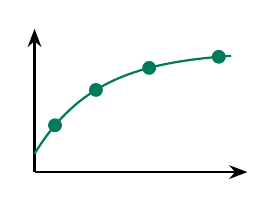
\begin{tikzpicture}[x=0.52cm,y=0.52cm]
        \draw[-{Stealth}, thick] (0,0) -- (5.2,0);
        \draw[-{Stealth}, thick] (0,0) -- (0,3.5);
        \draw[emphasis, thick] plot[smooth, domain=0:4.8] (\x,{0.45+2.5*(1-exp(-0.65*\x))});
        \foreach \x in {0.5,1.5,2.8,4.5} {
          \pgfmathsetmacro{\yt}{0.45+2.5*(1-exp(-0.65*\x))}
          \fill[emphasis] (\x,\yt) circle (2.5pt);
        }
      \end{tikzpicture}
    \column{0.31\textwidth}
      \centering
      {\fontsize{34}{38}\selectfont\con{3}}\par
      \vspace{3pt}
      \textbf{用功能干预限定解释}
      \vspace{6pt}
      \begin{tikzpicture}[node distance=0.38cm]
        \node[purplebox, text width=2.8cm] (rank) {重要性排序};
        \node[warmbox, text width=2.8cm, below=of rank] (prune) {定向剪枝};
        \node[greenbox, text width=2.8cm, below=of prune] (damage) {任务损伤};
        \draw[arr] (rank) -- (prune);
        \draw[strongarr] (prune) -- (damage);
      \end{tikzpicture}
  \end{columns}
  \vspace{7pt}
  \centering\HL{\textbf{定义、估计、训练轨迹、功能干预与稳健性共同构成可核验的证据体系。}}
  \note{
    第一项原则是区分实现误差、统计误差和数值误差。实现正确不代表估计无偏，估计无偏也不代表路径积分足够精确；三类问题需要不同的参考与判据。任何后续结构解释都应建立在测量可信度已经确认的基础上。\par
    第二项原则是保留训练时间维度。终点模型只能描述最终分布，不能区分重要参数在训练早期形成、后期重组或仅在终点偶然出现。纵向 checkpoint、集中度轨迹和集合重合共同用于描述结构形成过程。\par
    第三项原则是用功能性干预限制结论强度。相关性、集中度和稳定排序可以支持描述性结论；只有定向剪枝在多比例、多 seed 和随机基线下产生可重复损伤差异，才能进一步支持功能性表述。\par
    三项原则对应论文实验的逻辑顺序：测量校准、动态结构分析和功能验证，随后由消融与结论—证据映射界定外部有效性和可复核性。
  }
\end{frame}

% 29
\begin{frame}{参考文献}
  \begin{thebibliography}{9}
    \small
    \bibitem{project}
      Parameter Importance Project.
      \newblock 参数重要性研究实验计划与统一数学规格.
      \newblock Internal research documents, 2026.

    \bibitem{hoeffding1948}
      W. Hoeffding.
      \newblock A Class of Statistics with Asymptotically Normal Distribution.
      \newblock \emph{The Annals of Mathematical Statistics}, 19(3):293--325, 1948.

    \bibitem{sundararajan2017}
      M. Sundararajan, A. Taly, and Q. Yan.
      \newblock Axiomatic Attribution for Deep Networks.
      \newblock \emph{ICML}, PMLR 70:3319--3328, 2017.

    \bibitem{biderman2023}
      S. Biderman et al.
      \newblock Pythia: A Suite for Analyzing Large Language Models Across Training and Scaling.
      \newblock \emph{ICML}, PMLR 202:2397--2430, 2023.

    \bibitem{molchanov2019}
      P. Molchanov et al.
      \newblock Importance Estimation for Neural Network Pruning.
      \newblock \emph{CVPR}, 11264--11272, 2019.
  \end{thebibliography}
  \note{
    Hoeffding（1948）系统建立了 U-statistic 理论。核心思想是对不同样本组成的对称核函数求平均，从而构造目标总体量的无偏估计；本项目删除梯度自乘项的做法属于该框架的二阶情形。\par
    Sundararajan、Taly 与 Yan（2017）提出 Integrated Gradients，以输入空间路径积分满足 sensitivity 与 completeness 等归因公理。本项目研究的是参数空间中的实际更新端点，研究对象不同，但路径积分和完备性检查提供了重要方法参照。\par
    Biderman 等（2023）的 Pythia 模型族提供多个参数规模和训练 checkpoint，支持跨训练时间与模型规模的分析。Molchanov 等（2019）代表基于梯度/Taylor 近似的神经网络剪枝重要性研究，为 Stage 7 的传统基线和功能评价提供背景。\par
    内部数学规格负责确定本项目的目标量、符号、权重和判定边界；外部文献提供统计理论、归因思想、开放模型与剪枝方法背景。引用相关工作不意味着本项目与其研究对象完全相同，差异需在论文方法部分明确说明。
  }
\end{frame}

% 30
\begin{frame}{研究问题与讨论}
  \vspace{5pt}
  \centering
  {\Large\bfseries 参数重要性的形成过程，\par
   能否成为连接优化动态与泛化能力的中间表征？}
  \vspace{16pt}
  \begin{tikzpicture}[node distance=1.1cm]
    \node[flowbox, text width=3.2cm] (opt) {优化动态\\梯度与更新};
    \node[greenbox, text width=3.2cm, right=of opt] (importance) {重要性结构\\轨迹与分工};
    \node[purplebox, text width=3.2cm, right=of importance] (generalization) {模型能力\\功能与泛化};
    \draw[strongarr] (opt) -- (importance);
    \draw[strongarr] (importance) -- (generalization);
  \end{tikzpicture}
  \vfill
  {\Large\HL{感谢聆听 · Q\&A}}
  \note{
    最终研究问题是，参数重要性的形成过程能否作为连接优化动态与模型功能的中间表征。优化动态包括梯度、优化器状态和实际参数更新；重要性结构包括逐参数贡献、层级分布、集中度和随训练变化的稳定集合；模型功能则通过语言模型损失、下游任务性能和剪枝损伤评价。\par
    “中间表征”并不预设重要性是唯一机制解释。研究将检验三项可证伪关系：重要性估计是否在统计与数值上可信；重要性轨迹是否随模型规模和训练路线稳定变化；重要性排序是否预测受控剪枝造成的功能损伤。任一关系不成立，结论都应相应收缩。\par
    讨论可分为四类问题：无偏估计依赖哪些独立性假设；路径贡献对 probe set 和求积规则有多敏感；训练路线比较如何控制计算预算；剪枝干预能够支持何种程度的功能或因果表述。对应的公式推导与指标定义列在后续附录页。
  }
\end{frame}

\appendix

% 31
\begin{frame}{附录｜技术推导与指标定义}
  \centering
  {\Large\bfseries 技术细节与判读口径}
  \vspace{16pt}
  \begin{tikzpicture}[node distance=0.62cm]
    \node[flowbox, text width=2.8cm] (bias) {raw 正偏\\为何出现 $\sigma^2/B$};
    \node[greenbox, text width=2.8cm, right=of bias] (u) {U-statistic\\等权与加权形式};
    \node[purplebox, text width=2.8cm, right=of u] (path) {路径完备性\\为何贡献可求和};
    \node[warmbox, text width=2.8cm, right=of path] (metrics) {指标词典\\统计与功能判据};
    \draw[arr] (bias) -- (u);
    \draw[arr] (u) -- (path);
    \draw[arr] (path) -- (metrics);
  \end{tikzpicture}
  \vspace{14pt}
  \begin{block}{附录内容}
    包括 raw 正偏、U-statistic 权重、路径完备性及统计指标的正式定义。
  \end{block}
  \note{
    附录不计入主讲时间，用于回答方法定义和统计口径方面的追问。第一部分从二阶矩分解推导 raw estimator 的正偏；第二部分给出等权与按有效 token 数加权的 U-statistic；第三部分由链式法则和微积分基本定理推导路径完备性；第四部分集中定义误差、相关性、集中度和剪枝损伤指标。\par
    四页附录对应四类常见问题：为何 raw 有偏；microbatch 大小不一致时如何加权；逐参数路径贡献为何能够求和为端点损失差；不同指标各自支持何种结论。引用附录时应同时说明相关假设，避免只展示公式而忽略定义域和统计单位。
  }
\end{frame}

% 32
\begin{frame}{附录｜raw estimator 正偏的二阶矩分解}
  \textbf{同一 minibatch 的平均梯度平方为何不等于 $\mu_k^2$？}
  \begin{align*}
    \bar g_k &= \frac{1}{B}\sum_{i=1}^{B} g_k(z_i),
    &\mathbb E[\bar g_k]&=\mu_k,\\
    \mathbb E[\bar g_k^2]
      &=\operatorname{Var}(\bar g_k)+\mathbb E[\bar g_k]^2,
    &\operatorname{Var}(\bar g_k)&=\frac{\sigma_k^2}{B},\\
    \Rightarrow\quad
    \mathbb E[\bar g_k^2]&=\mu_k^2+\frac{\sigma_k^2}{B}.&&
  \end{align*}
  \begin{columns}[T]
    \column{0.48\textwidth}
      \begin{exampleblock}{标量例子}
        \[
          \mu=2,\quad \sigma^2=9,\quad B=9
          \;\Rightarrow\; \mathbb E[\bar g^2]=5
        \]
      \end{exampleblock}
    \column{0.48\textwidth}
      \begin{block}{判别预测}
        \begin{itemize}
          \item 真目标：$\mu^2=4$
          \item raw 额外增加 1
          \item $B$ 增大时偏差按 $1/B$ 衰减
        \end{itemize}
      \end{block}
  \end{columns}
  \keyline{double sample 与 U-statistic 均通过排除同一样本的自乘项实现无偏化。}
  \note{
    $g_k(z_i)$ 是样本 $z_i$ 对参数 $k$ 的梯度，$\bar g_k$ 是 $B$ 个样本梯度的算术平均。若样本独立同分布，则 $\mathbb E[\bar g_k]=\mu_k$，$\operatorname{Var}(\bar g_k)=\sigma_k^2/B$。\par
    二阶矩恒等式 $\mathbb E[X^2]=\operatorname{Var}(X)+\mathbb E[X]^2$ 将平均梯度平方的期望分成方差项与均值平方。目标是总体平均梯度的平方 $\mu_k^2$，而 raw estimator 的期望多出 $\sigma_k^2/B$；该项非负，因此产生系统性正偏。\par
    标量例中 $\mu=2$、$\sigma^2=9$、$B=9$，目标为 $\mu^2=4$，raw 的期望为 $4+9/9=5$。增加 batch size 会减小方差项，但有限 $B$ 下仍然有偏。\par
    若样本之间相关，则 $\operatorname{Var}(\bar g)$ 还包含成对协方差：正相关通常使偏差大于 $\sigma^2/B$，负相关可能减小偏差。此时需要使用实际抽样设计对应的方差表达式，不能沿用独立样本简式。
  }
\end{frame}

% 33
\begin{frame}{附录｜等权与加权 U-statistic}
  \begin{columns}[T]
    \column{0.48\textwidth}
      \textbf{等权 microbatch}
      \[
        \widehat{\mu_k^2}^{\,U}
        =\frac{S_{1,k}^2-S_{2,k}}{M(M-1)}
        =\frac{1}{M(M-1)}\sum_{m\ne n}g_{m,k}g_{n,k}
      \]
      \begin{itemize}
        \item $S_{1,k}=\sum_m g_{m,k}$
        \item $S_{2,k}=\sum_m g_{m,k}^2$
        \item $M\ge2$；交换顺序结果不变
      \end{itemize}
    \column{0.48\textwidth}
      \textbf{不等有效 token 数}
      \[
        \widehat{\mu_k^2}^{\,U_w}
        =\frac{G_{1,k}^2-G_{2,k}}{N_1^2-N_2}
      \]
      \begin{itemize}
        \item $G_{1,k}=\sum_m b_m g_{m,k}$
        \item $G_{2,k}=\sum_m b_m^2 g_{m,k}^2$
        \item $N_1=\sum_m b_m$，$N_2=\sum_m b_m^2$
      \end{itemize}
  \end{columns}
  \vspace{6pt}
  \begin{exampleblock}{一致性检查}
    当所有 $b_m$ 相等时，加权式退化为等权式；分母必须严格为正。
  \end{exampleblock}
  \keyline{U-statistic 的权重必须与训练损失的样本或有效 token 口径一致。}
  \note{
    等权式假设每个 microbatch 梯度 $g_{m,k}$ 代表相同数量、相同权重的统计单位。$S_{1,k}^2-S_{2,k}$ 等于所有 $m\ne n$ 有序交叉乘积之和，分母 $M(M-1)$ 是对应有序对数量。交换 microbatch 顺序不应改变结果。\par
    语言模型训练中，不同 microbatch 可能因 padding 或序列截断而包含不同的有效 token 数。令 $b_m$ 为第 $m$ 个 microbatch 的有效 token 数，若损失按 token 平均，则各梯度对总体均值的权重应与 $b_m$ 一致。$G_1$ 是加权梯度和，$G_2$ 删除加权自乘项，$N_1^2-N_2$ 是不同 microbatch 权重乘积的总和。\par
    分母必须严格为正，这要求至少存在两个正权重 microbatch。若所有 $b_m$ 相等，加权式应严格退化为等权式；该性质是实现测试的重要 oracle。若训练损失按序列而非 token 平均，则 $b_m$ 应改为相应的有效样本权重。\par
    无偏解释仍依赖不同 microbatch 的独立性或零交叉协方差。权重修正解决的是统计单位不一致，并不能自动消除数据重复、序列相关或采样分布变化带来的偏差。
  }
\end{frame}

% 34
\begin{frame}{附录｜路径积分完备性的推导}
  \textbf{固定线性路径 $\Gamma(\alpha)=\Theta_0+\alpha\Delta\Theta$ 与标量损失 $\mathcal L$。}
  \begin{align*}
    \frac{d}{d\alpha}\mathcal L(\Gamma(\alpha))
      &=\nabla_\Theta \mathcal L(\Gamma(\alpha))^\top\Delta\Theta,\\
    \mathcal L(\Theta_1)-\mathcal L(\Theta_0)
      &=\int_0^1\sum_k
        \partial_k\mathcal L(\Gamma(\alpha))\,\Delta\theta_k\,d\alpha.
  \end{align*}
  定义 $C_k^{\mathrm{path}}=-\Delta\theta_k\int_0^1\partial_k\mathcal L(\Gamma(\alpha))d\alpha$，则
  \[
    \boxed{\sum_k C_k^{\mathrm{path}}
      =\mathcal L(\Theta_0)-\mathcal L(\Theta_1)}
  \]
  \begin{center}
  \begin{tikzpicture}[node distance=0.65cm]
    \node[flowbox, text width=2.8cm] (path) {固定端点与路径};
    \node[greenbox, text width=2.8cm, right=of path] (grad) {沿路径积分梯度};
    \node[purplebox, text width=2.8cm, right=of grad] (sum) {逐参数贡献求和};
    \node[warmbox, text width=2.8cm, right=of sum] (loss) {得到端点 loss 差};
    \draw[arr] (path) -- (grad);
    \draw[arr] (grad) -- (sum);
    \draw[strongarr] (sum) -- (loss);
  \end{tikzpicture}
  \end{center}
  \note{
    线性路径定义为 $\Gamma(\alpha)=\Theta_0+\alpha\Delta\Theta$，其中 $\Delta\Theta=\Theta_1-\Theta_0$。由链式法则，损失对路径参数的导数等于参数梯度与路径方向的内积：$d\mathcal L/d\alpha=\nabla_\Theta\mathcal L^\top\Delta\Theta$。\par
    对 $\alpha$ 从 0 积到 1，并使用微积分基本定理，可得到端点损失差 $\mathcal L(\Theta_1)-\mathcal L(\Theta_0)$。将内积按参数坐标 $k$ 展开，再把负号并入贡献定义，就得到 $\sum_k C_k^{\mathrm{path}}=\mathcal L(\Theta_0)-\mathcal L(\Theta_1)$。负号约定使损失下降对应正的总贡献。\par
    连续积分下，完备性是定义和可微条件共同给出的恒等式，不是经验相关性。离散求积时，完备性残差衡量所有参数贡献之和与实际端点 loss 差之间的差异，但一个较小的标量残差仍可能掩盖逐参数正负误差抵消，因此必须同时检查向量误差和排序。\par
    残差异常时，应依次核验端点是否来自同一次真实更新、probe set 与模型模式是否固定、路径节点是否正确、求积权重是否归一化，以及浮点累积精度是否充分。若路径穿过不可微点，自动微分给出的次梯度也需在解释中说明。
  }
\end{frame}

% 35
\begin{frame}{附录｜指标定义、用途与统计单位}
  \vspace{4pt}
  \begin{center}
  \begin{tabular}{lll}
    \toprule
    指标 & 回答的问题 & 主要使用阶段 \\
    \midrule
    Bias & 估计均值偏离参考多少？ & Stage 2 \\
    Variance / MSE & 重复波动与综合误差多大？ & Stage 2 \\
    Pearson / Spearman & 数值或排序是否一致？ & Stage 2--3 \\
    top-$k$ overlap & 关键参数集合是否恢复？ & Stage 2--6 \\
    Gini / entropy & 重要性分布是否集中？ & Stage 5--8 \\
    HHI / 有效参数数 & 质量由多少参数承载？ & Stage 5--8 \\
    Damage AUC & 剪枝全过程造成多少功能损伤？ & Stage 7 \\
    配对置信区间 & 路线或配置差异是否稳定？ & Stage 6--9 \\
    \bottomrule
  \end{tabular}
  \end{center}
  \vspace{8pt}
  \begin{block}{统计单位}
    参数坐标用于分布与排序，不充当独立重复；置信区间以 repetition、checkpoint、模型或 seed 为单位。
  \end{block}
  \keyline{估计误差、排序一致性、分布集中度与功能损伤对应不同证据层级。}
  \note{
    Bias 是估计量重复均值与参考值之差，反映系统误差；Variance 是估计量围绕自身均值的波动；MSE 是相对参考值的平方误差期望，等于 Bias 的平方加 Variance。三者共同评价数值准确性，MSE 较小不保证 Bias 为零。\par
    Pearson correlation 衡量两个数值向量的线性关系，对缩放和异常值敏感；Spearman correlation 对秩计算，衡量排序的单调一致性。top-$k$ overlap 只比较排名前 $k$ 的集合，通常定义为交集大小除以 $k$；它不评价集合内部次序，也不代表完整排序一致。\par
    对非负归一化份额 $p_k$，Gini 衡量整体不均衡程度；entropy $-\sum_k p_k\log p_k$ 越大表示越分散；HHI $\sum_k p_k^2$ 越大表示越集中；有效参数数 $1/\mathrm{HHI}$ 将集中度转换为等效的等权参数数量。这些指标需要明确负值处理和归一化方式。\par
    Damage AUC 是任务损伤对剪枝比例的积分，衡量整个剪枝区间的累计功能损伤。配对置信区间先在同一 seed、任务、checkpoint 或 mask 对内计算差值，再跨独立重复估计不确定性。参数坐标共享模型状态，不构成独立重复。\par
    常量向量使 Pearson 与 Spearman 的分母为零；零总质量使份额归一化不可定义；只有一个有效重复时无法估计重复间方差。此类结果应报告 NA、产生原因和受影响结论，不用任意常数替代。
  }
\end{frame}

\end{document}
